In a time-independent Hamiltonian scenario, neutron excited states are present
in the hadron source. These excited states decay and eventually only the ground state
remains. This effect manifests in the three-point function; there is a plateau in the
neutron energy. 
In our analysis, the Hamiltonian is time-dependent; excited states 
come from the hadron source but are also continuously produced by the time 
evolution, i.e., a fast-changing electric field. This time dependence could be
extracted from a time-dependent, expressed in Euclidean time, perturbation theory
analysis. A fit function would contain the effects from excited states from the hadron
source and the excited states generated by the electromagnetic perturbation, i.e.,
the time-varying electric field. Whereas in a time-independent Hamiltonian case there
is no inflection point shift, in our time-dependent case, one of the indicators 
of the excited state presence is a consistent shift in the inflection point. However, we argue 
that there is no significant slope variation between $t=6a$ and the inflection point 
in the three-window analysis. In the one-window analysis the shift in the inflection point is
not resolvable. At the same time, the slope values at $t=6a$ and at the shifted inflection point also
agree within uncertainties. Thus, \textcolor{red}{no excited state analysis is required for the results in our work}.

\subsection{Slope values at $t=6a$ for the connected diagrams in the 
3-window and 1-window analyses}
\label{ritardation_connected}
Significant retardation effects would be suggested by non-negligible deviations
of the slope at the shifted inflection point with respect to the slope at $t/a=6$. 
Our results show compatible slope values at these points. Note that in our three-
window analysis the fit of choice is $t/a=$ 5 to 7, and the slopes agree within 
uncertainties even though the inflection points are shifted to the right, as shown
in Figure~\ref{fig:shifinflecconn}.
%%%% extremal, position and slope, Multi point, connected diagrams%%%
\begin{table}[H]
\begin{center}
    \begin{tabular}{ | l | c | c | c |}
    \hline
     Fit range [$t/a$] & 5 to 7    & 4 to 8 & 3 to 9      \\ 
     \hline
        	Inflection point [$t/a$] &   6.43(24)         &      6.74(19)    &    7.28(13)   \\ \hline
        Extremal slope [$a^3$] &    -0.0127(77)        &     -0.0149(58)    &      -0.0194(42) \\ \hline
 	Slope at $t=6a$ [$a^3$] &    -0.0111(86)        &     -0.0109(68)   &     -0.0083(52)   \\ \hline
    
    \end{tabular}
\end{center}
\caption{Inflection points, extremal slope and slope at $t=6a$ for the $\chi^2$
linear fits for connected diagrams in the 3-window analysis with parabola minimum lift correction.}
\label{tab:Retardation3wMultiPoint}
\end{table}

%%%%%%%%%%%%%%%%%%%%%%%%%%%%%%%%%%%%%%

\begin{figure}[H]
  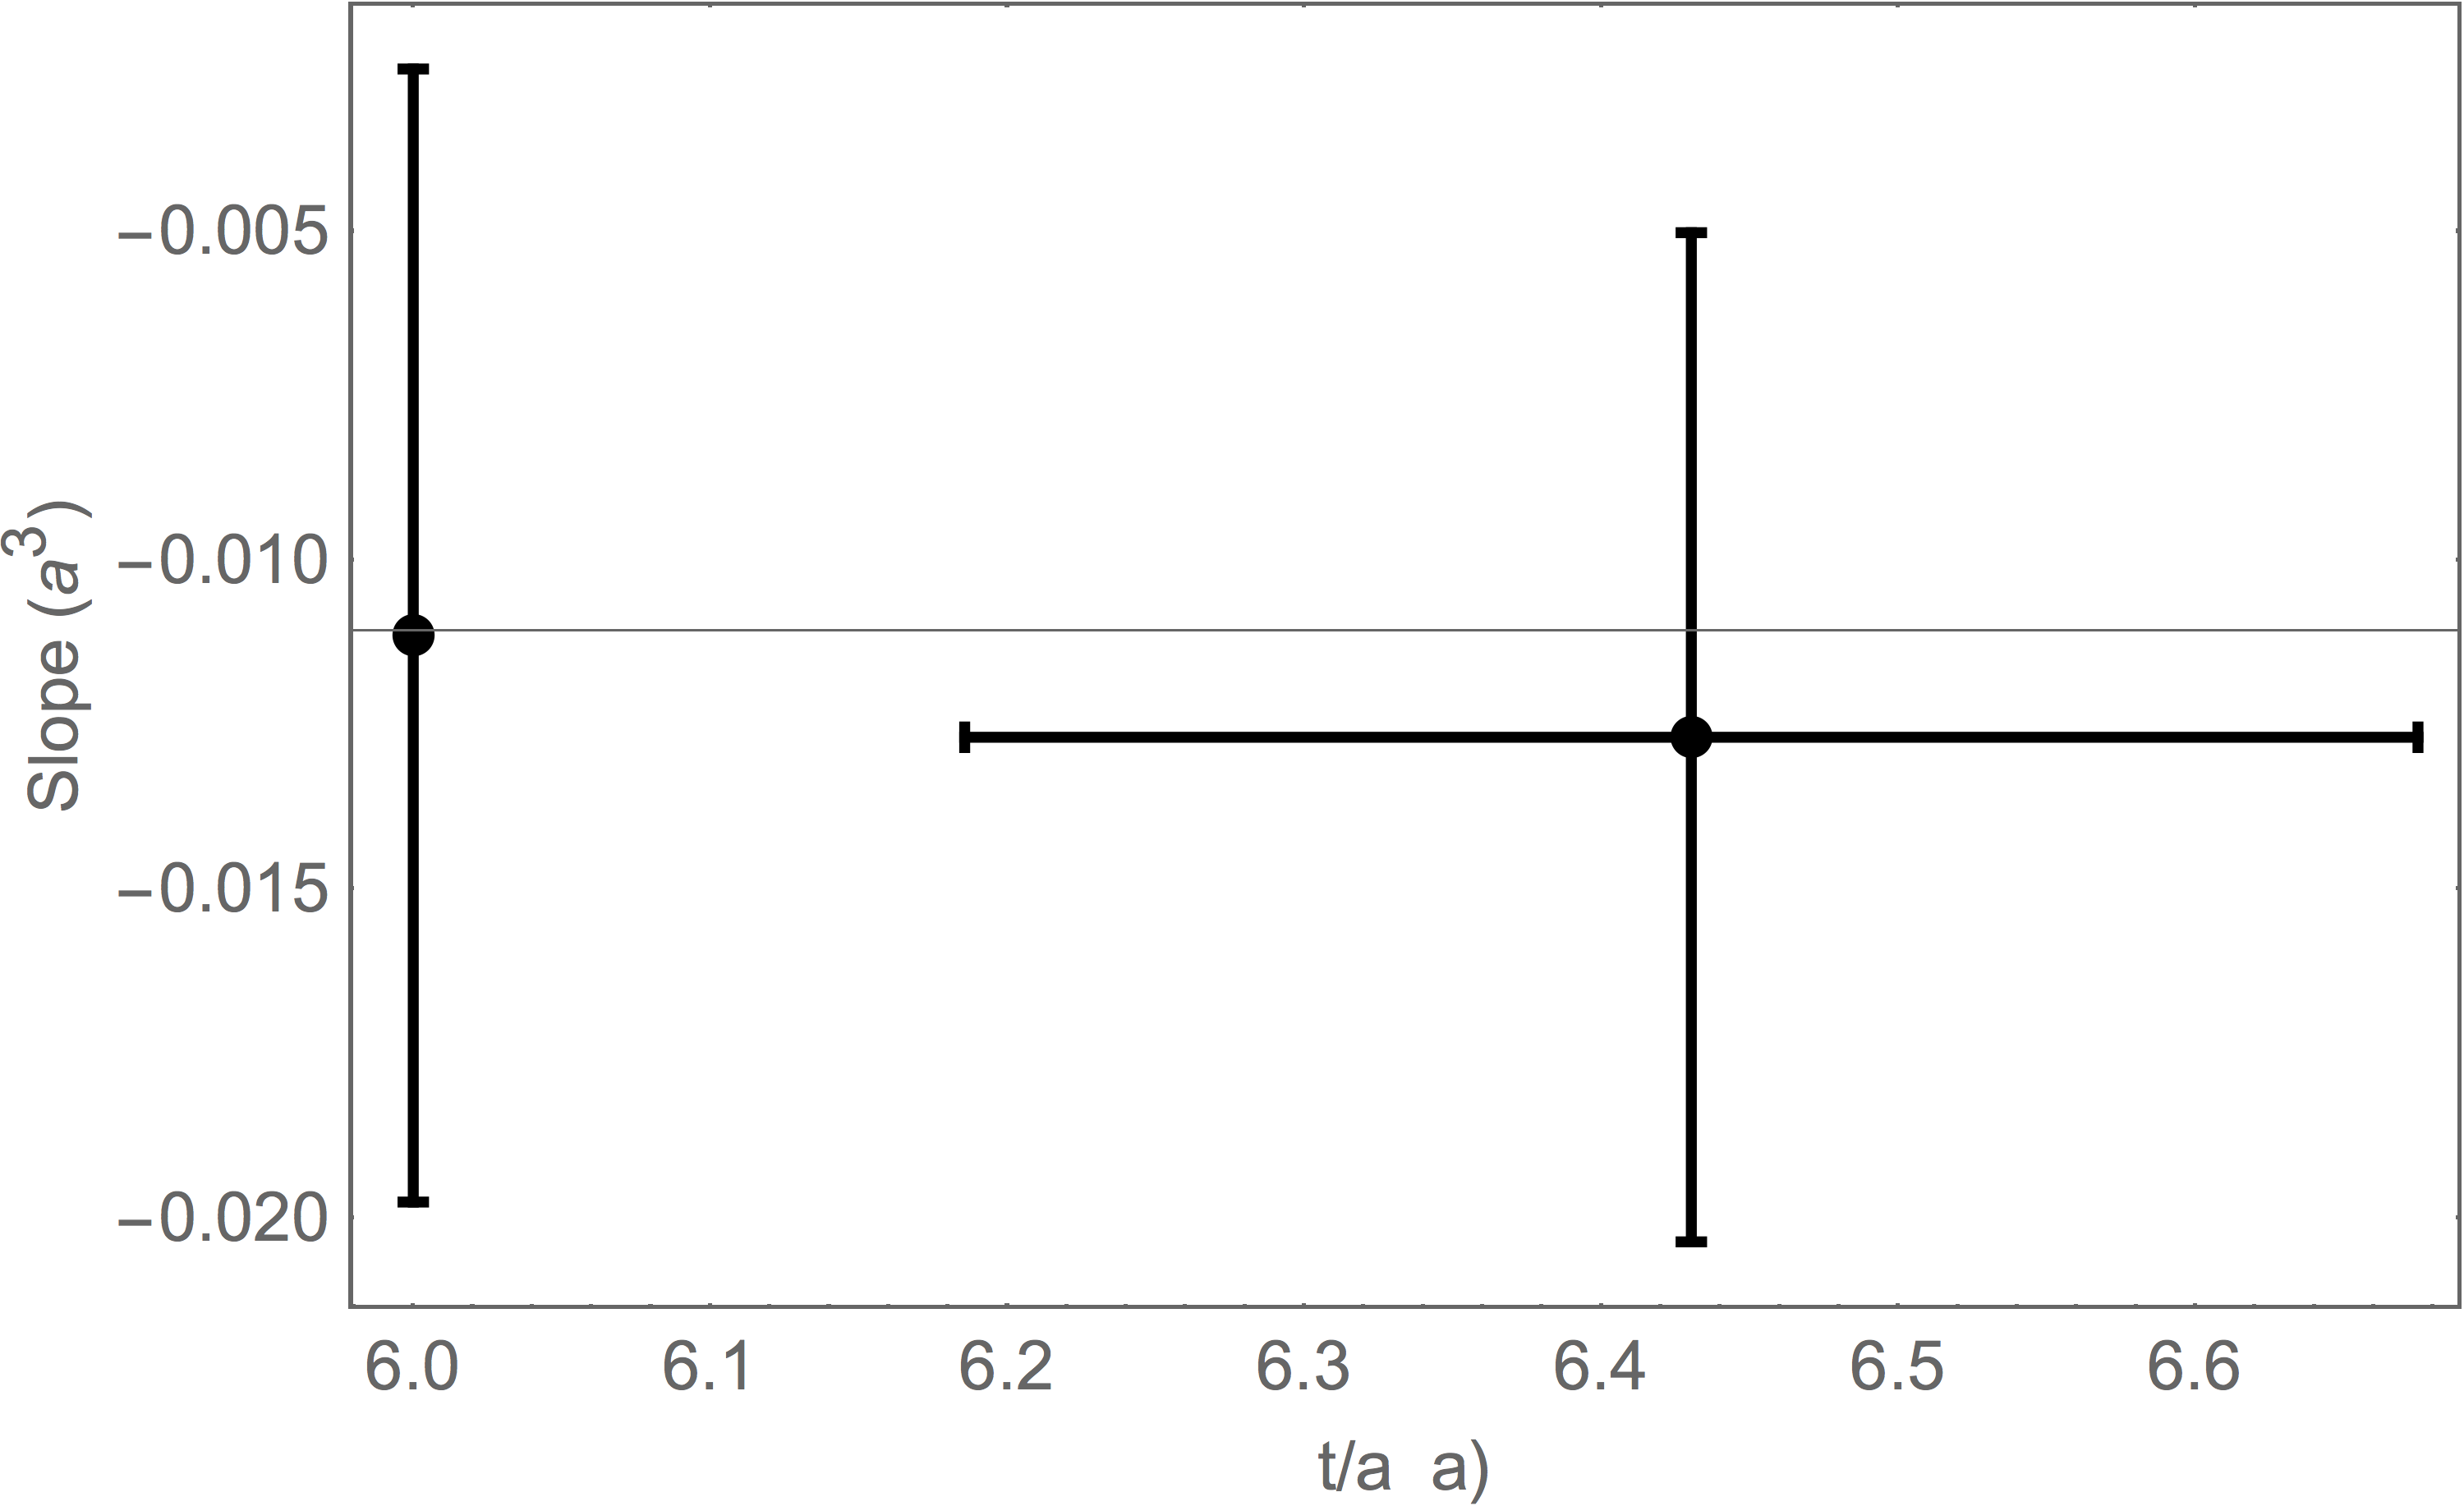
\includegraphics[width=.33\linewidth]{figures/3wC5-7Chi.png}
  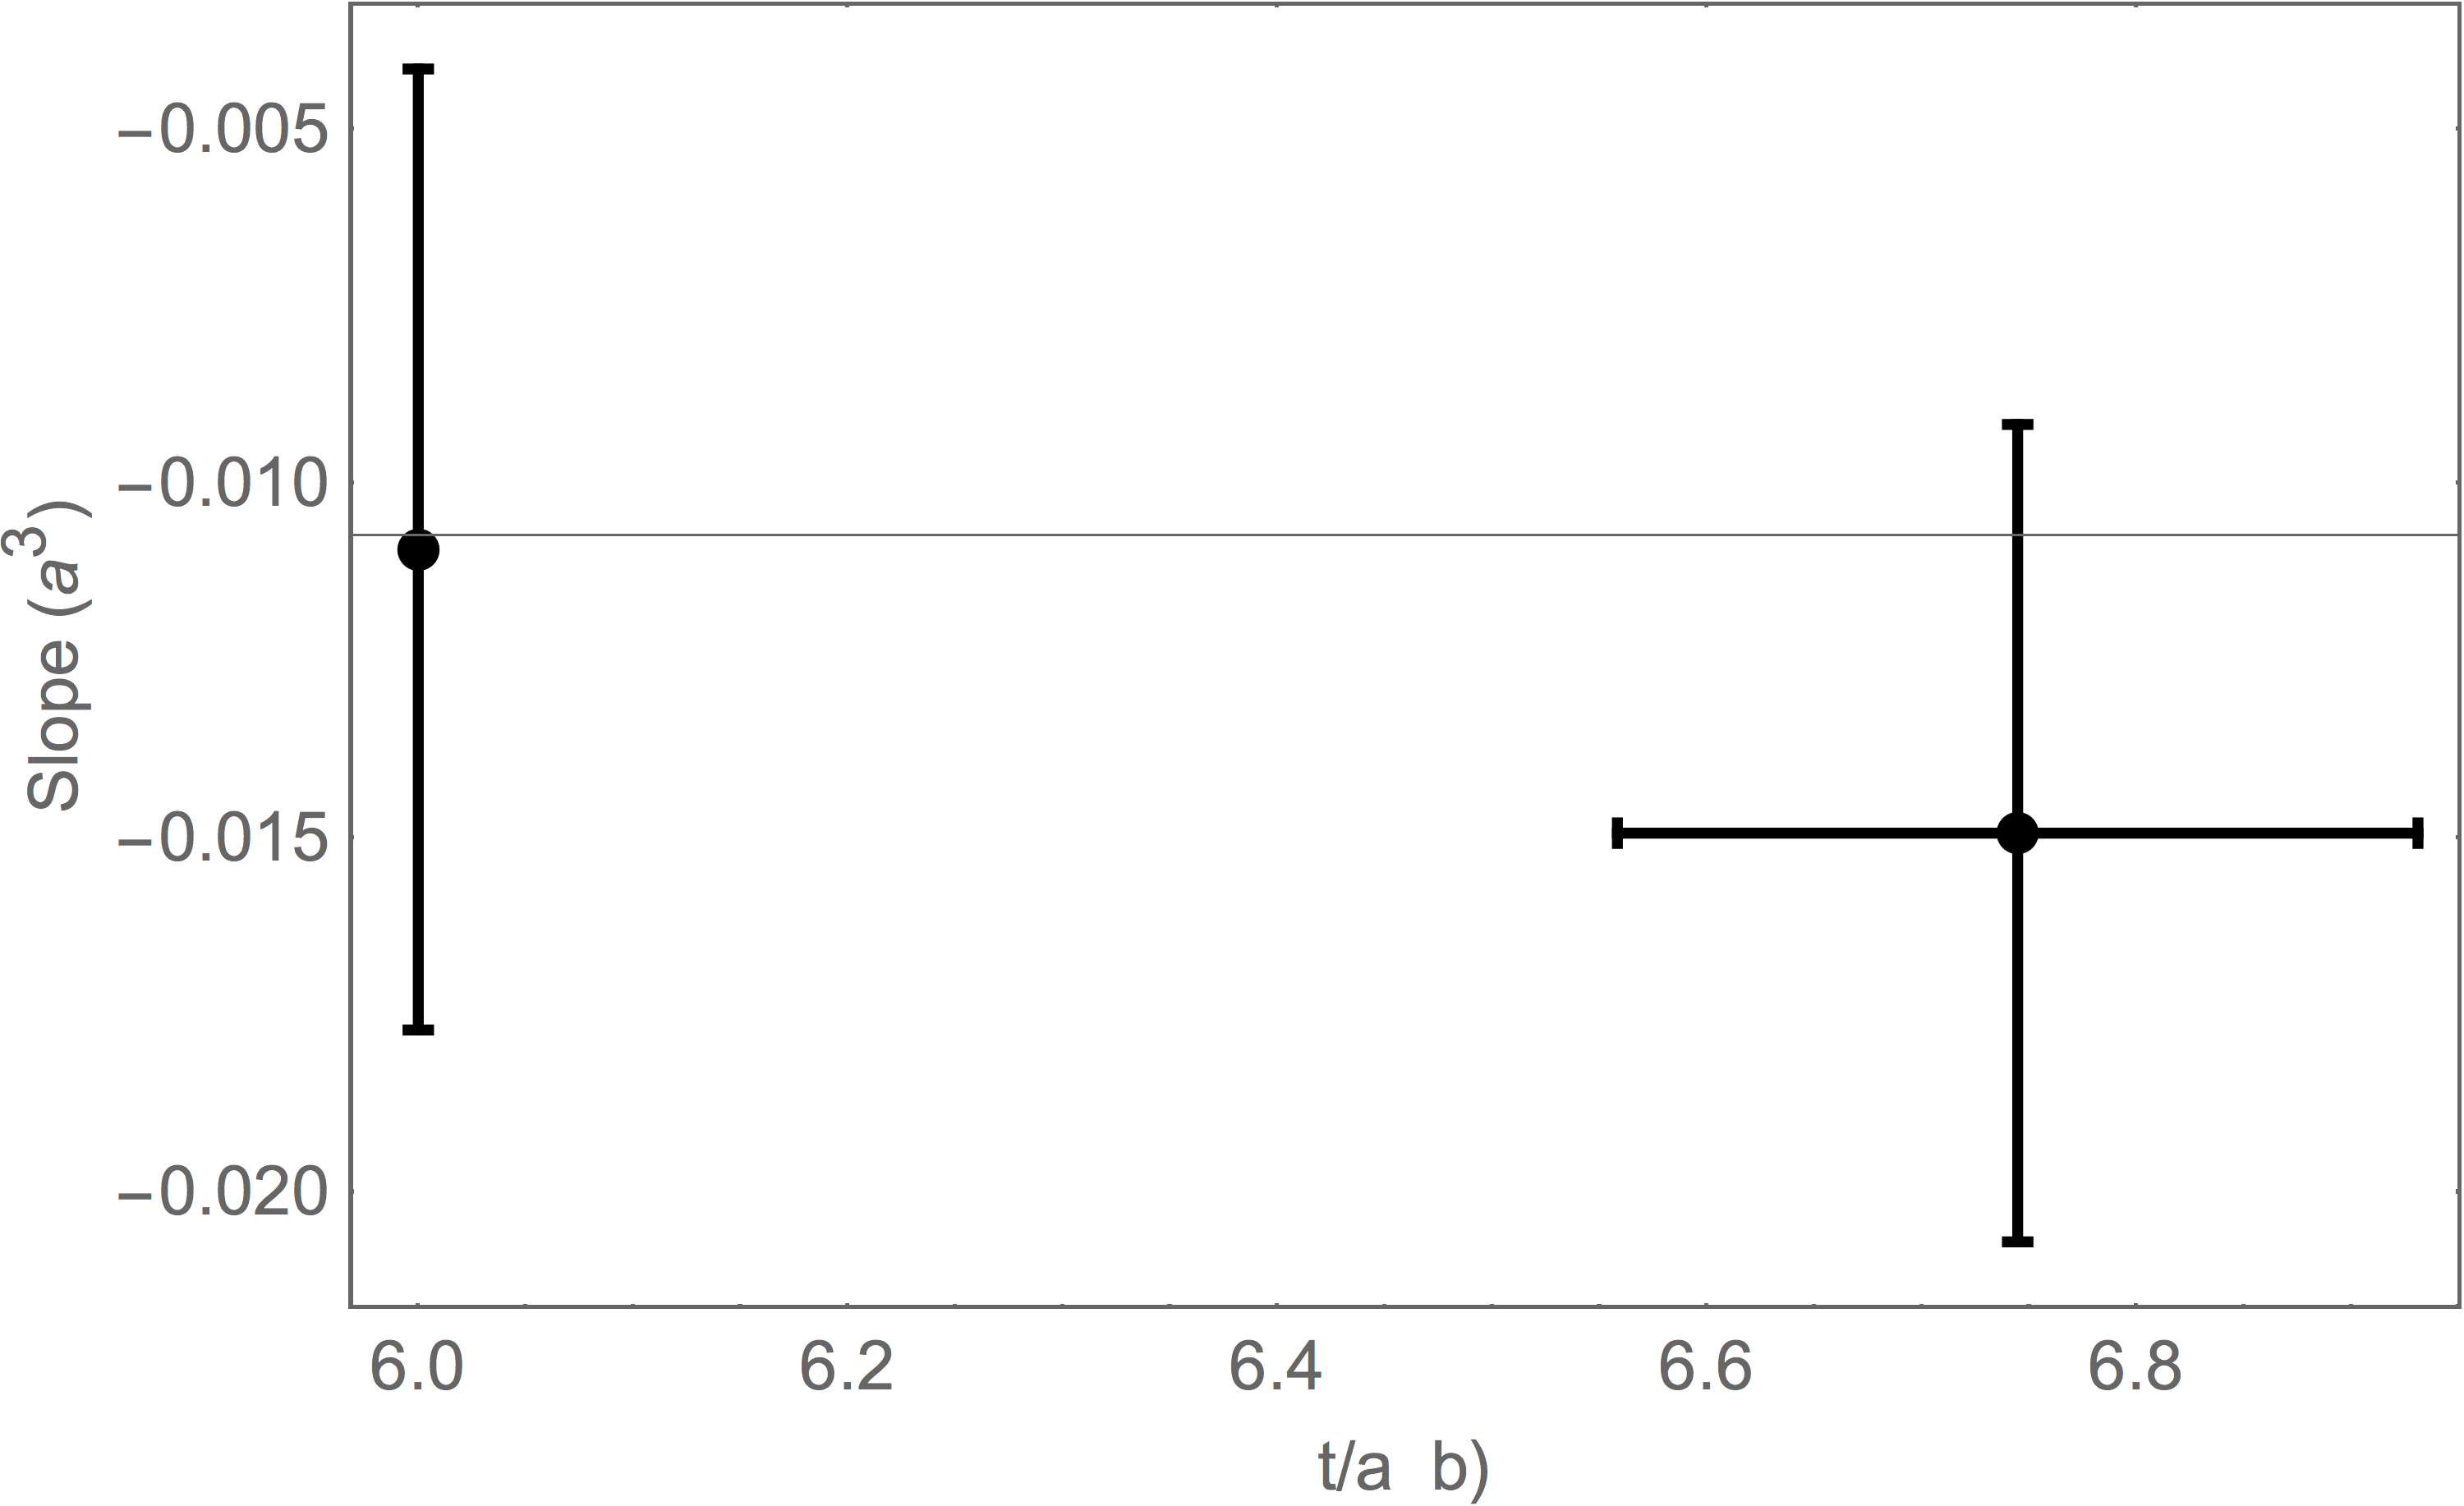
\includegraphics[width=.33\linewidth]{figures/3wC4-8Chi.png}
  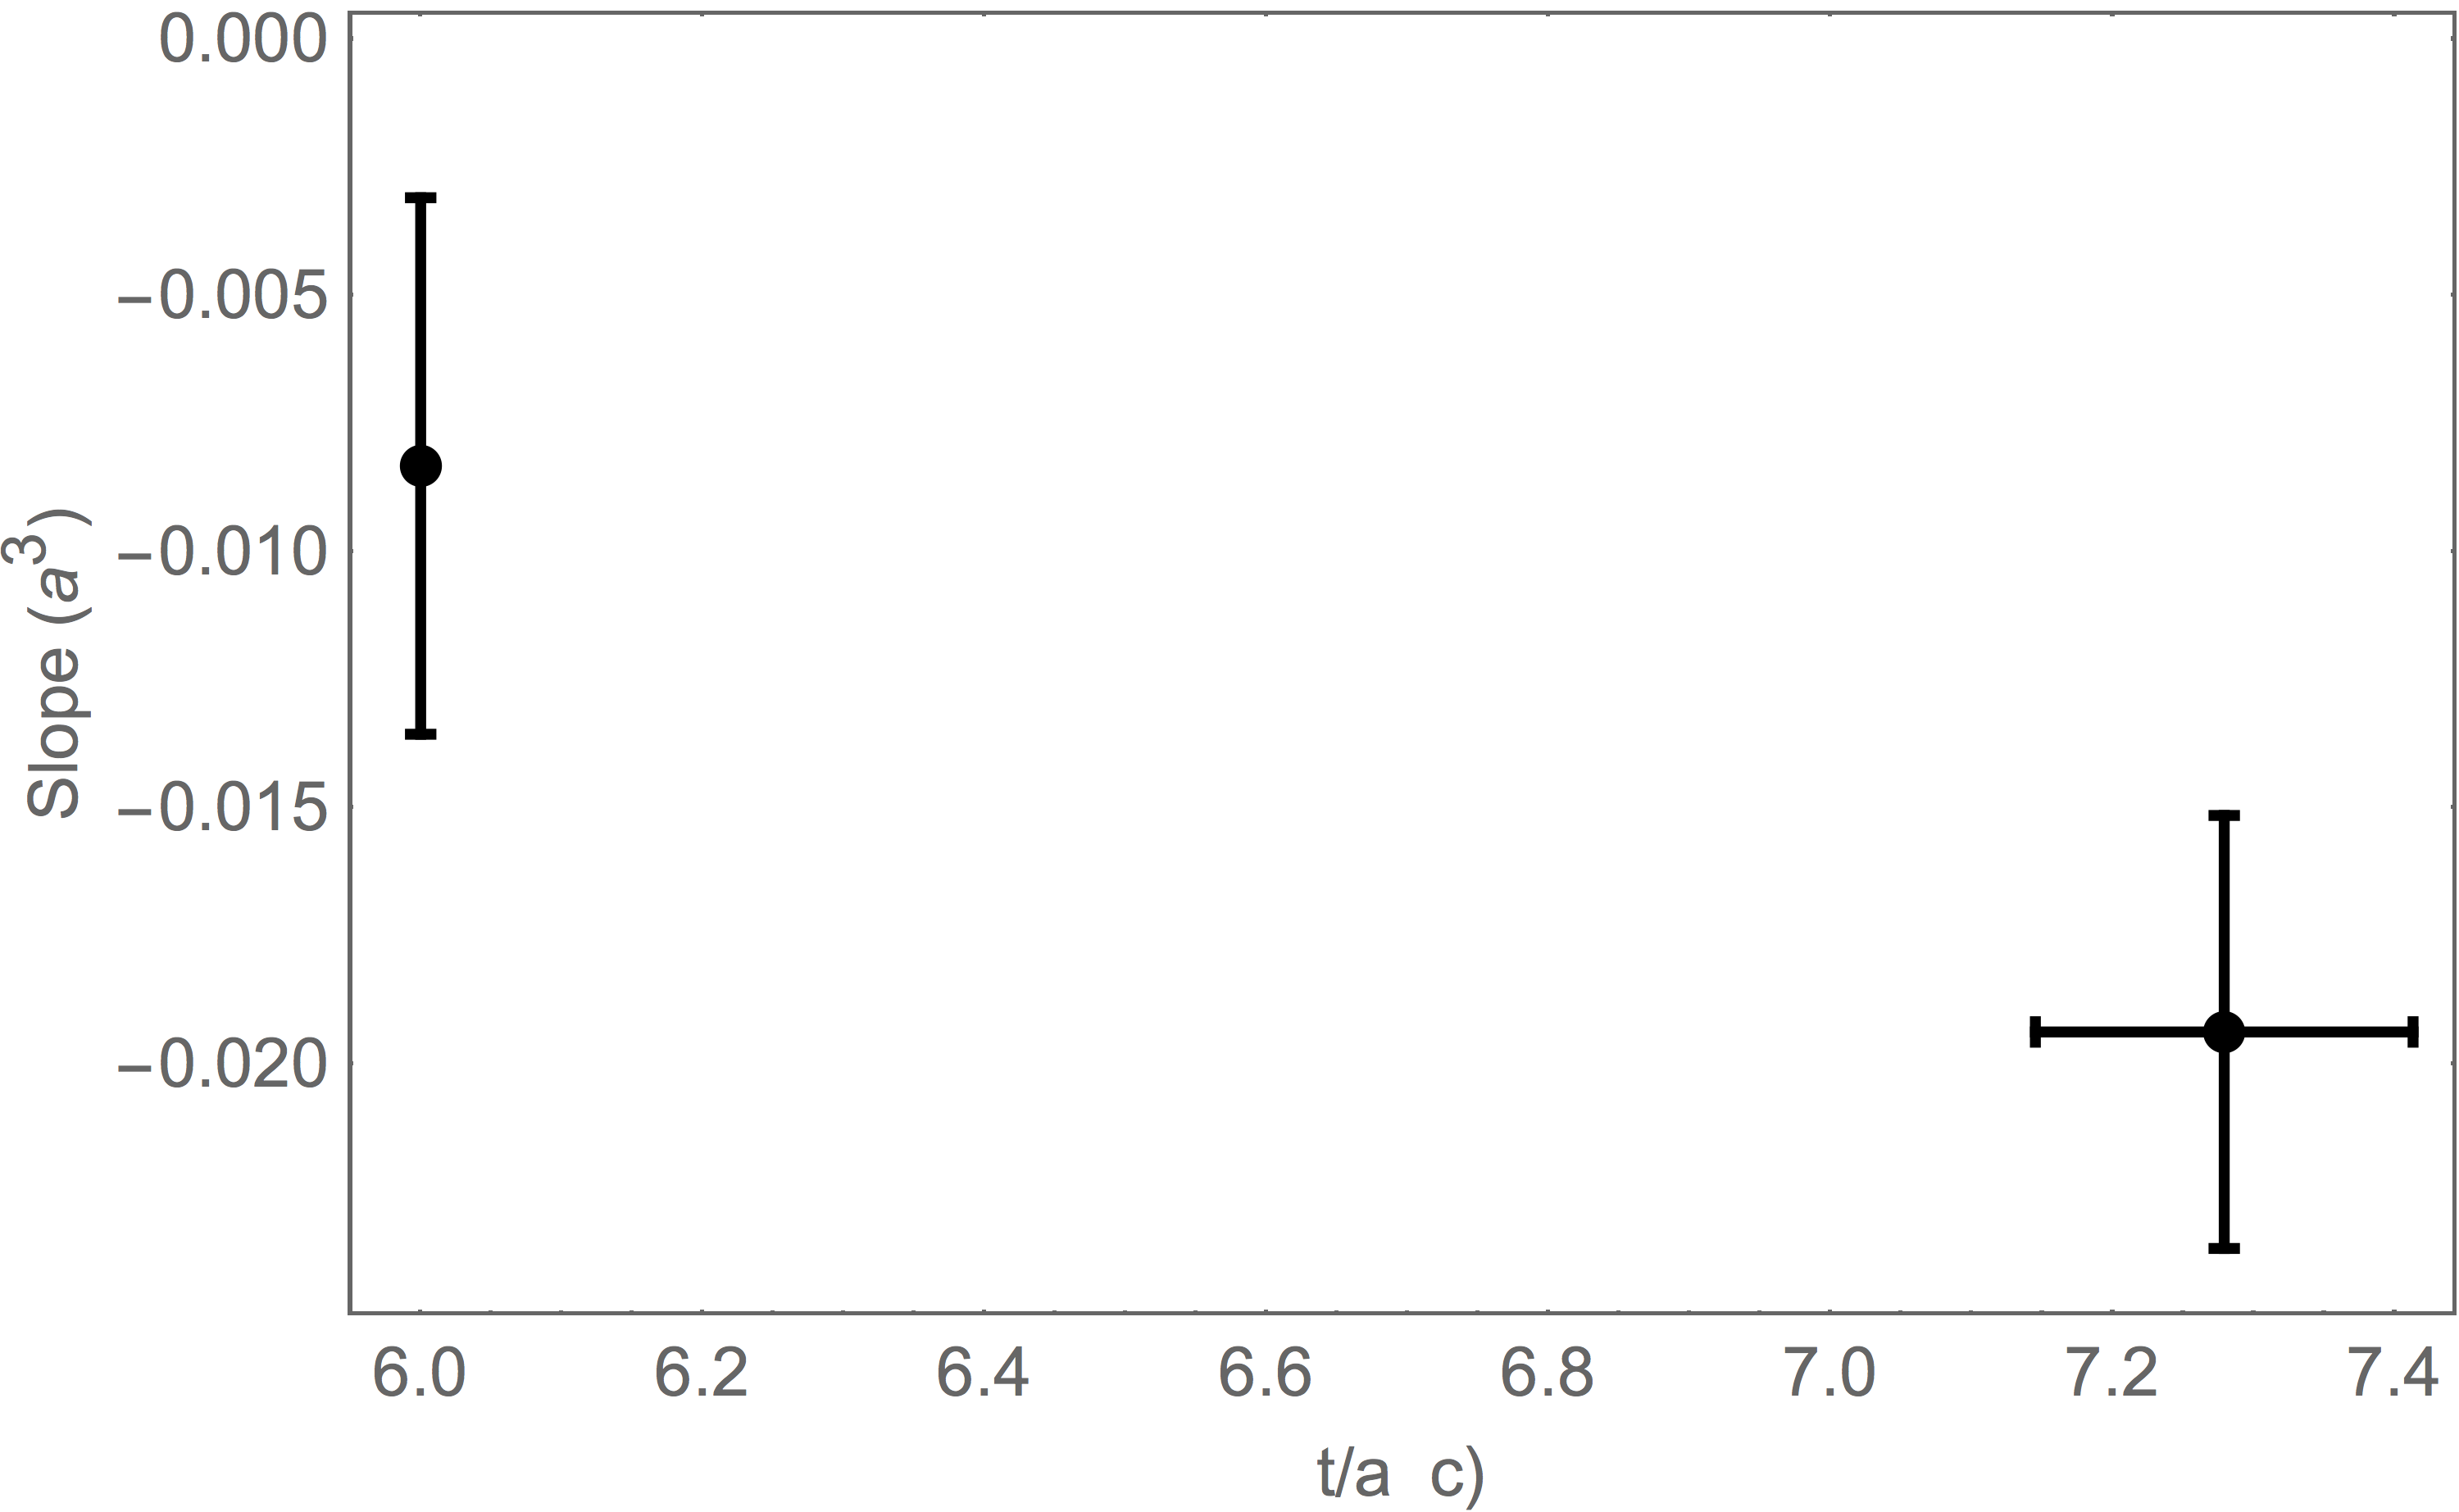
\includegraphics[width=.33\linewidth]{figures/3wC3-9Chi.png}
  \caption{Slope values at the shifted inflection points and at $t=6a$ for the
  connected diagrams. a) 5 to 7, b) 4 to 8, c) 3 to 9 $\chi^2$ fit ranges in the 
  three-window analysis.}
  \label{fig:shifinflecconn}
\end{figure}

Our one-window analysis also confirms that an excited state analysis can be avoided; 
the values of the slopes at the points of inflection also agree within uncertainties.
The results from table~\ref{tab:1walphaconnected} are show in figure~\ref{fig:1wshift_conn}.
\begin{figure}[H]
  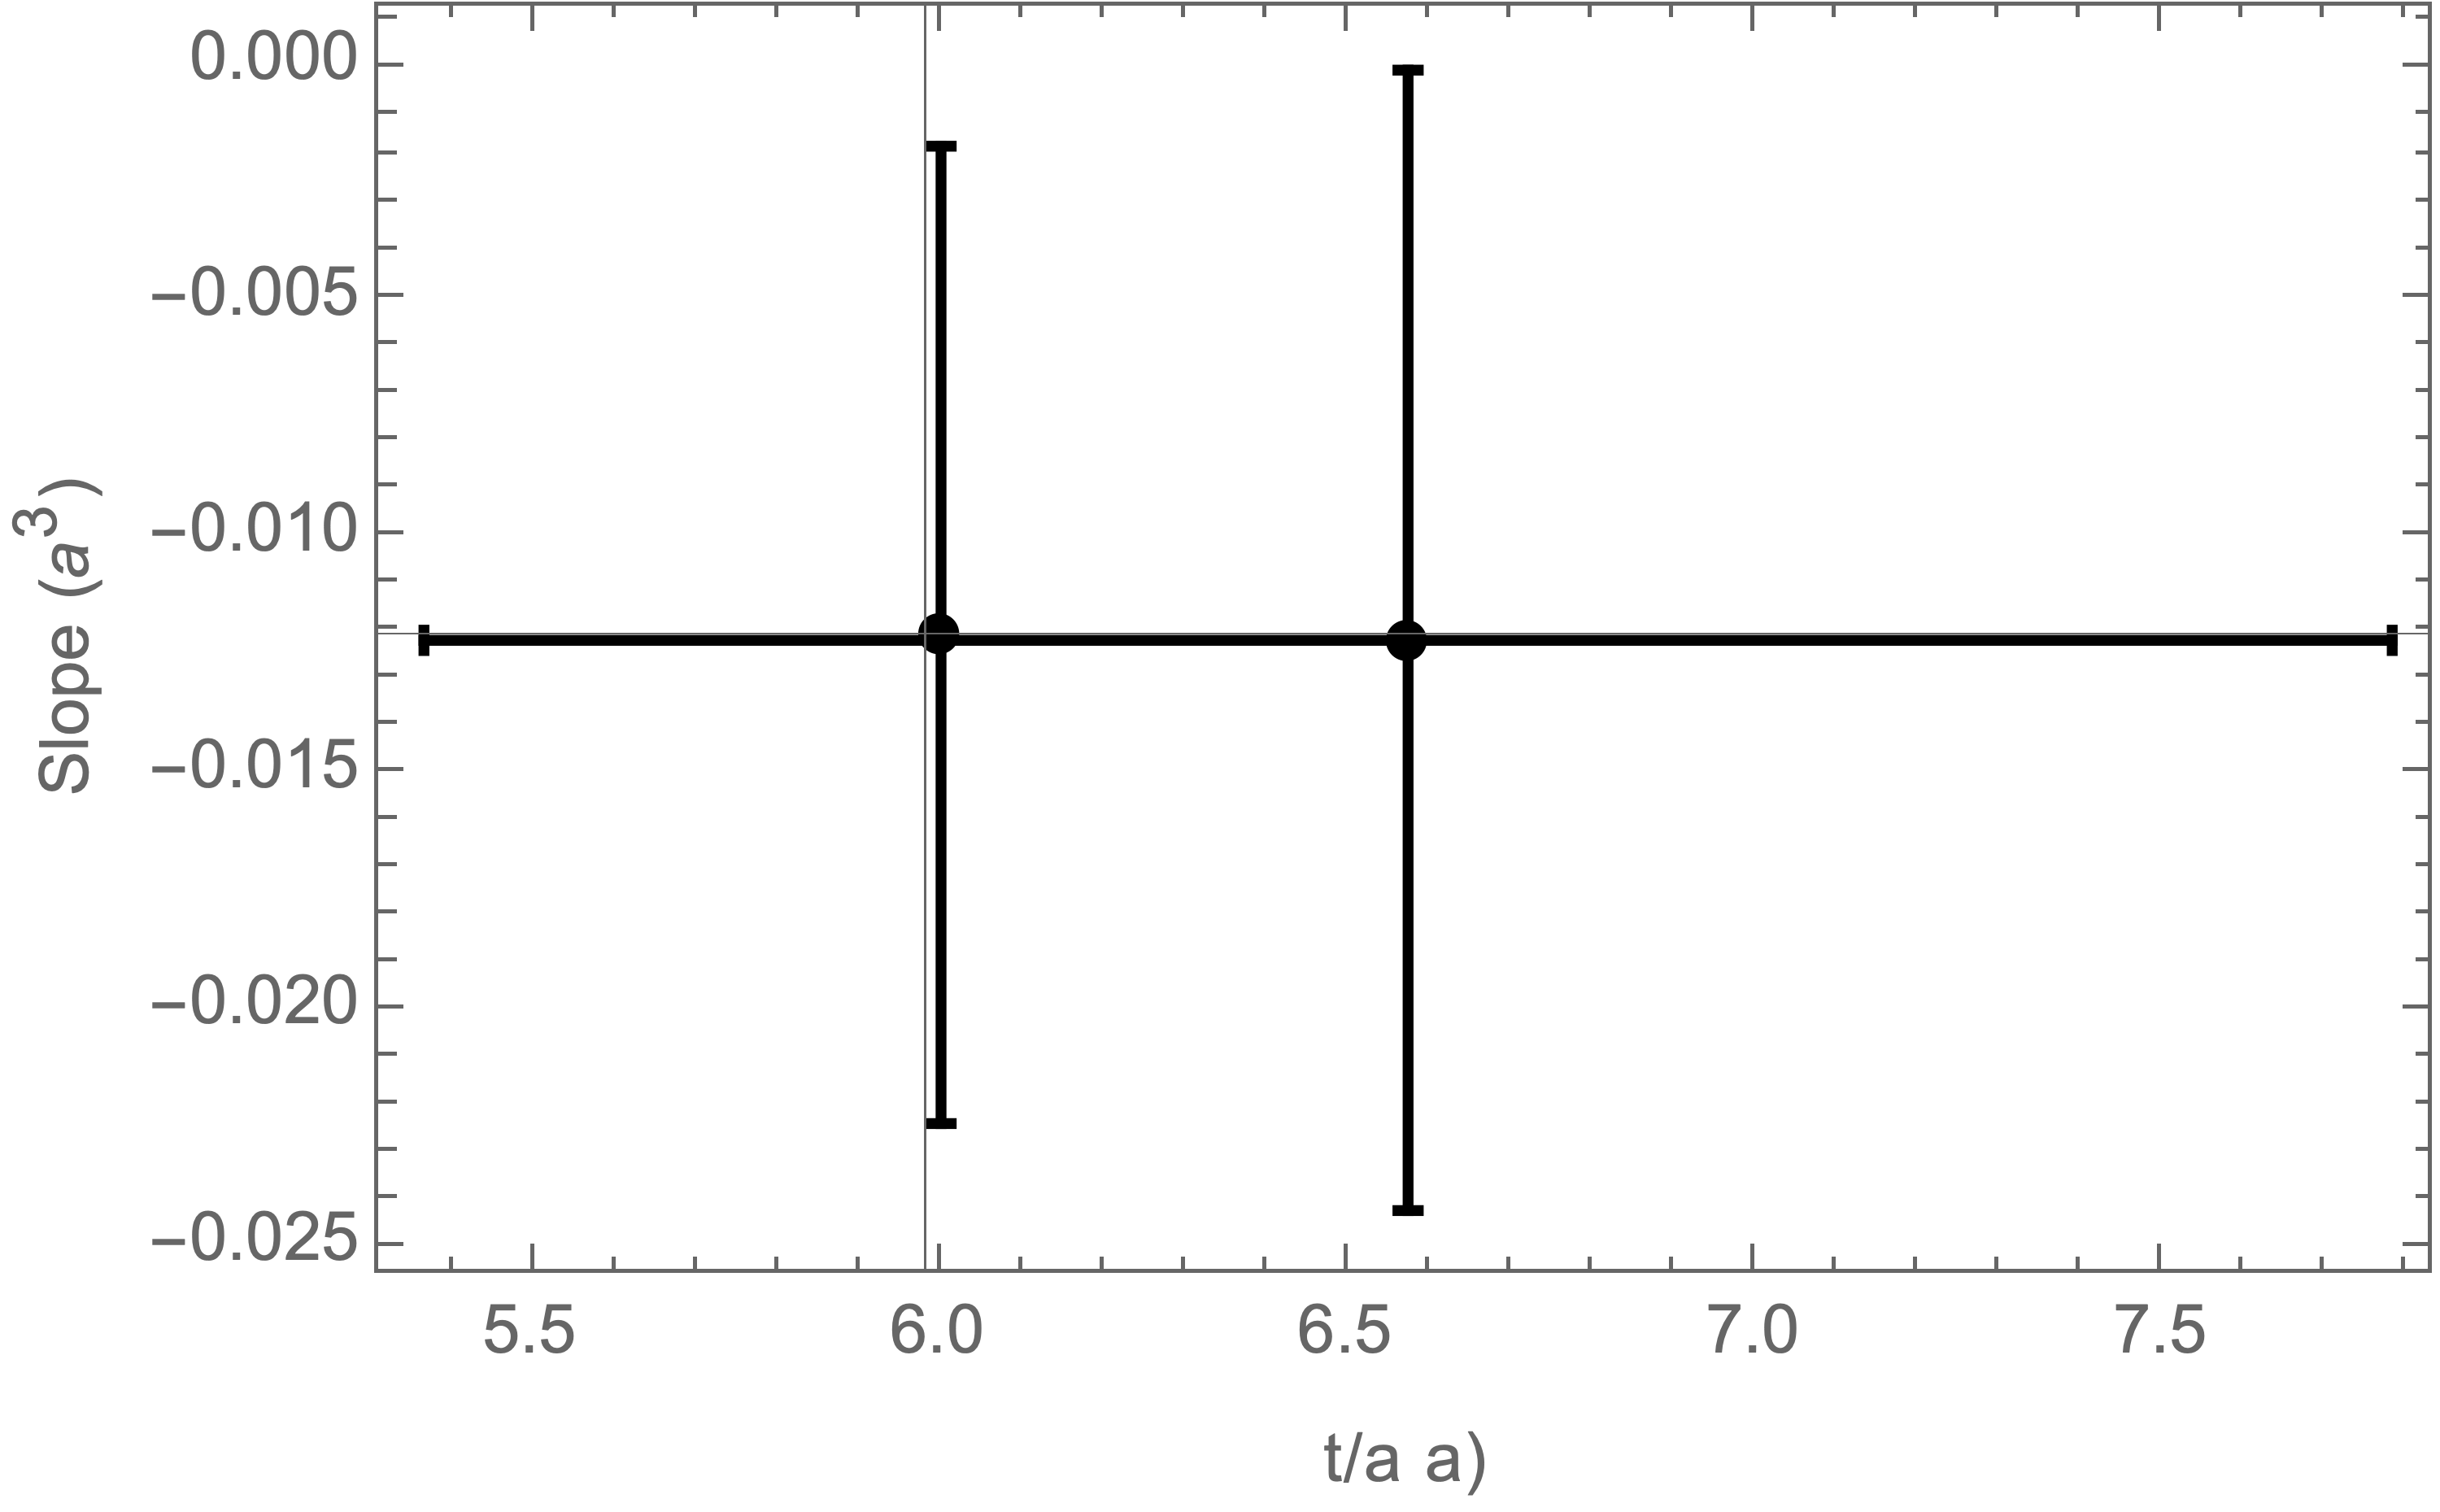
\includegraphics[width=.49\linewidth]{figures/1wC4-8Chi2021.png}
  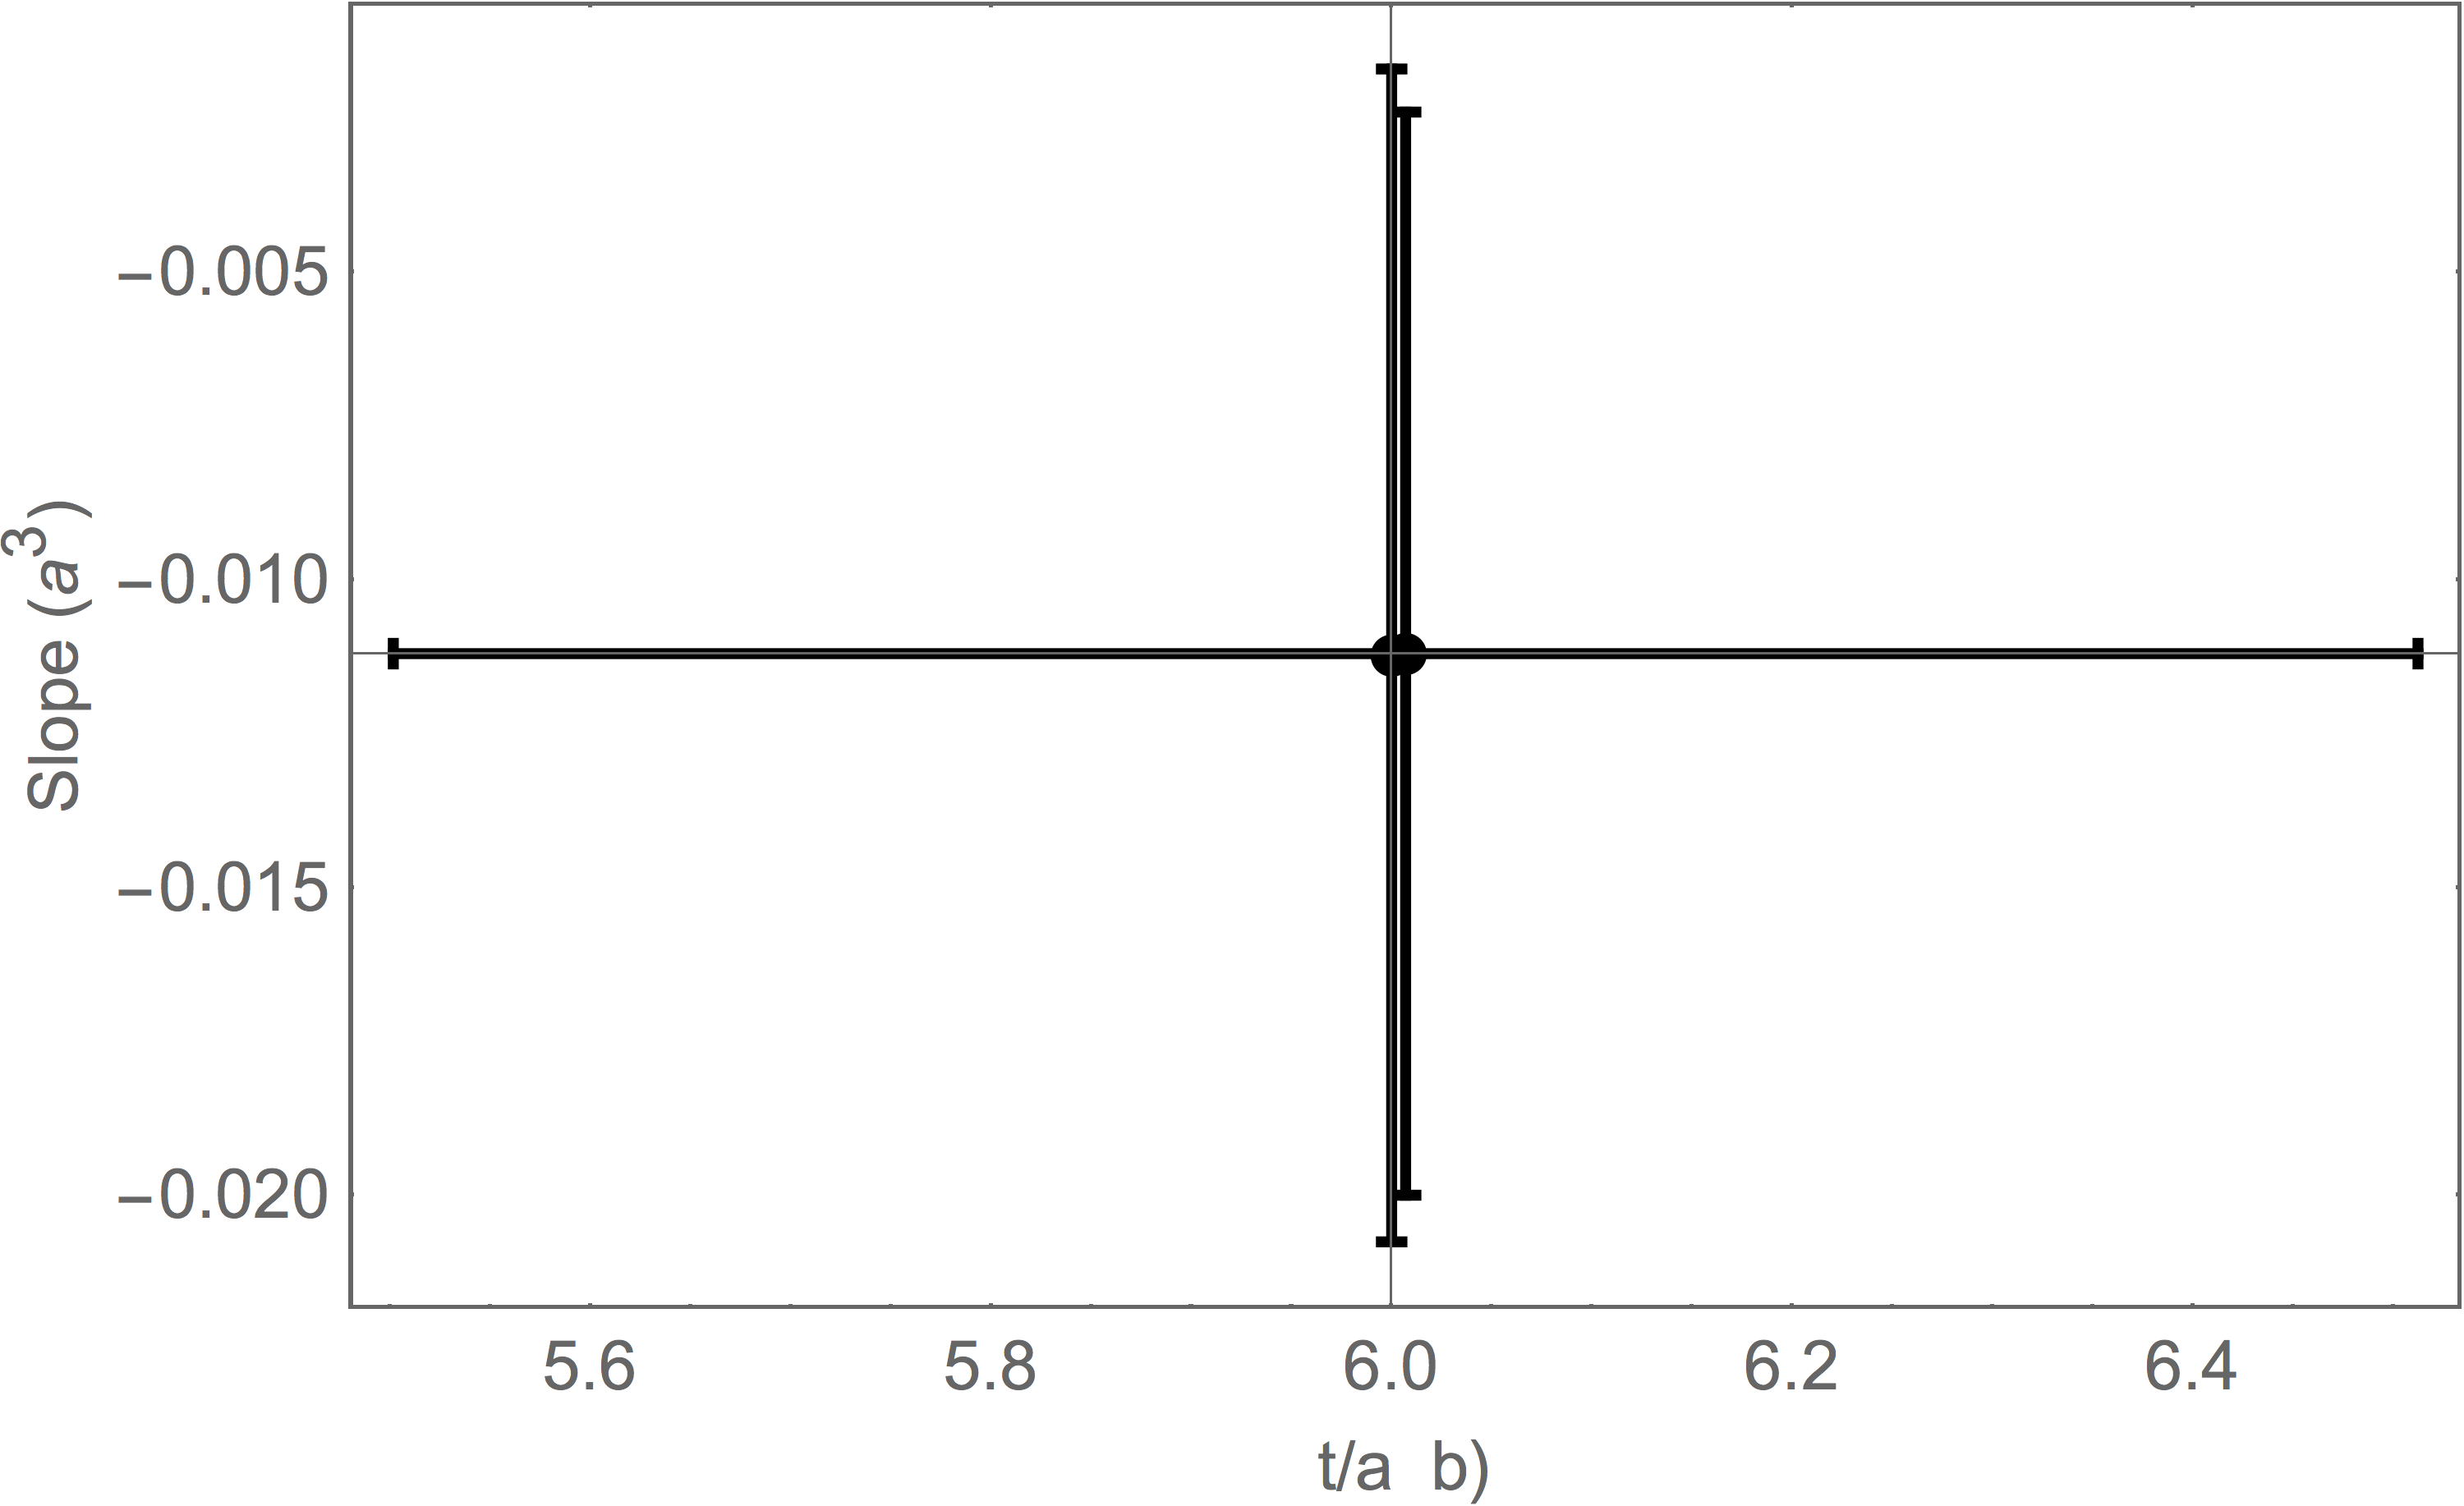
\includegraphics[width=.495\linewidth]{figures/1wC3-9Chi.png}
  \caption{Slope values for the $\chi^2$ fits, with and without a quadratic term. a) 4 to 8,
  b) 3-9 fit ranges for the connected diagrams in the one-window analysis}
  \label{fig:1wshift_conn}
\end{figure}
%%%%%%%%%%%%%%%%%%%%%%
\subsection{Slope values at $t=6a$ for all diagrams in the 3-window and
1-window  analyses}
The slope values at $t=6a$ and at the shifted inflection point also agree within uncertainties, 
as shown in fiigure~\ref{fig:shiftinflec_all}.
%%%% extremal, position and slope, Multi point, All diagrams%%%
\begin{table}[H]
\begin{center}
    \begin{tabular}{ | c | c | c | c |}
    \hline
     Fit range [$t/a$] & 5 to 7    & 4 to 8 & 3 to 9      \\ 
     \hline
   	Inflection point [$t/a$] &   6.99(39)         &      6.97(36)    &    7.12(34)   \\ \hline
        Extremal slope [$a^3$] &    -0.002(24)        &     0.001(19)    &      0.005(16) \\ \hline
 	Slope at $t=6a$ [$a^3$] &    0.010(21)        &     0.010(16)   &     0.016(14)   \\ \hline
    \end{tabular}
\end{center}
\caption{Inflection points, extremal slope and slope at $t=6a$ for the $\chi^2$
linear fits for connected diagrams in the 3-window analysis with parabola minimum lift correction.}
\label{tab:Retardation3wMultiPointAll}
\end{table}
%%%%%%%%%%%%%%
\begin{figure}[H]
  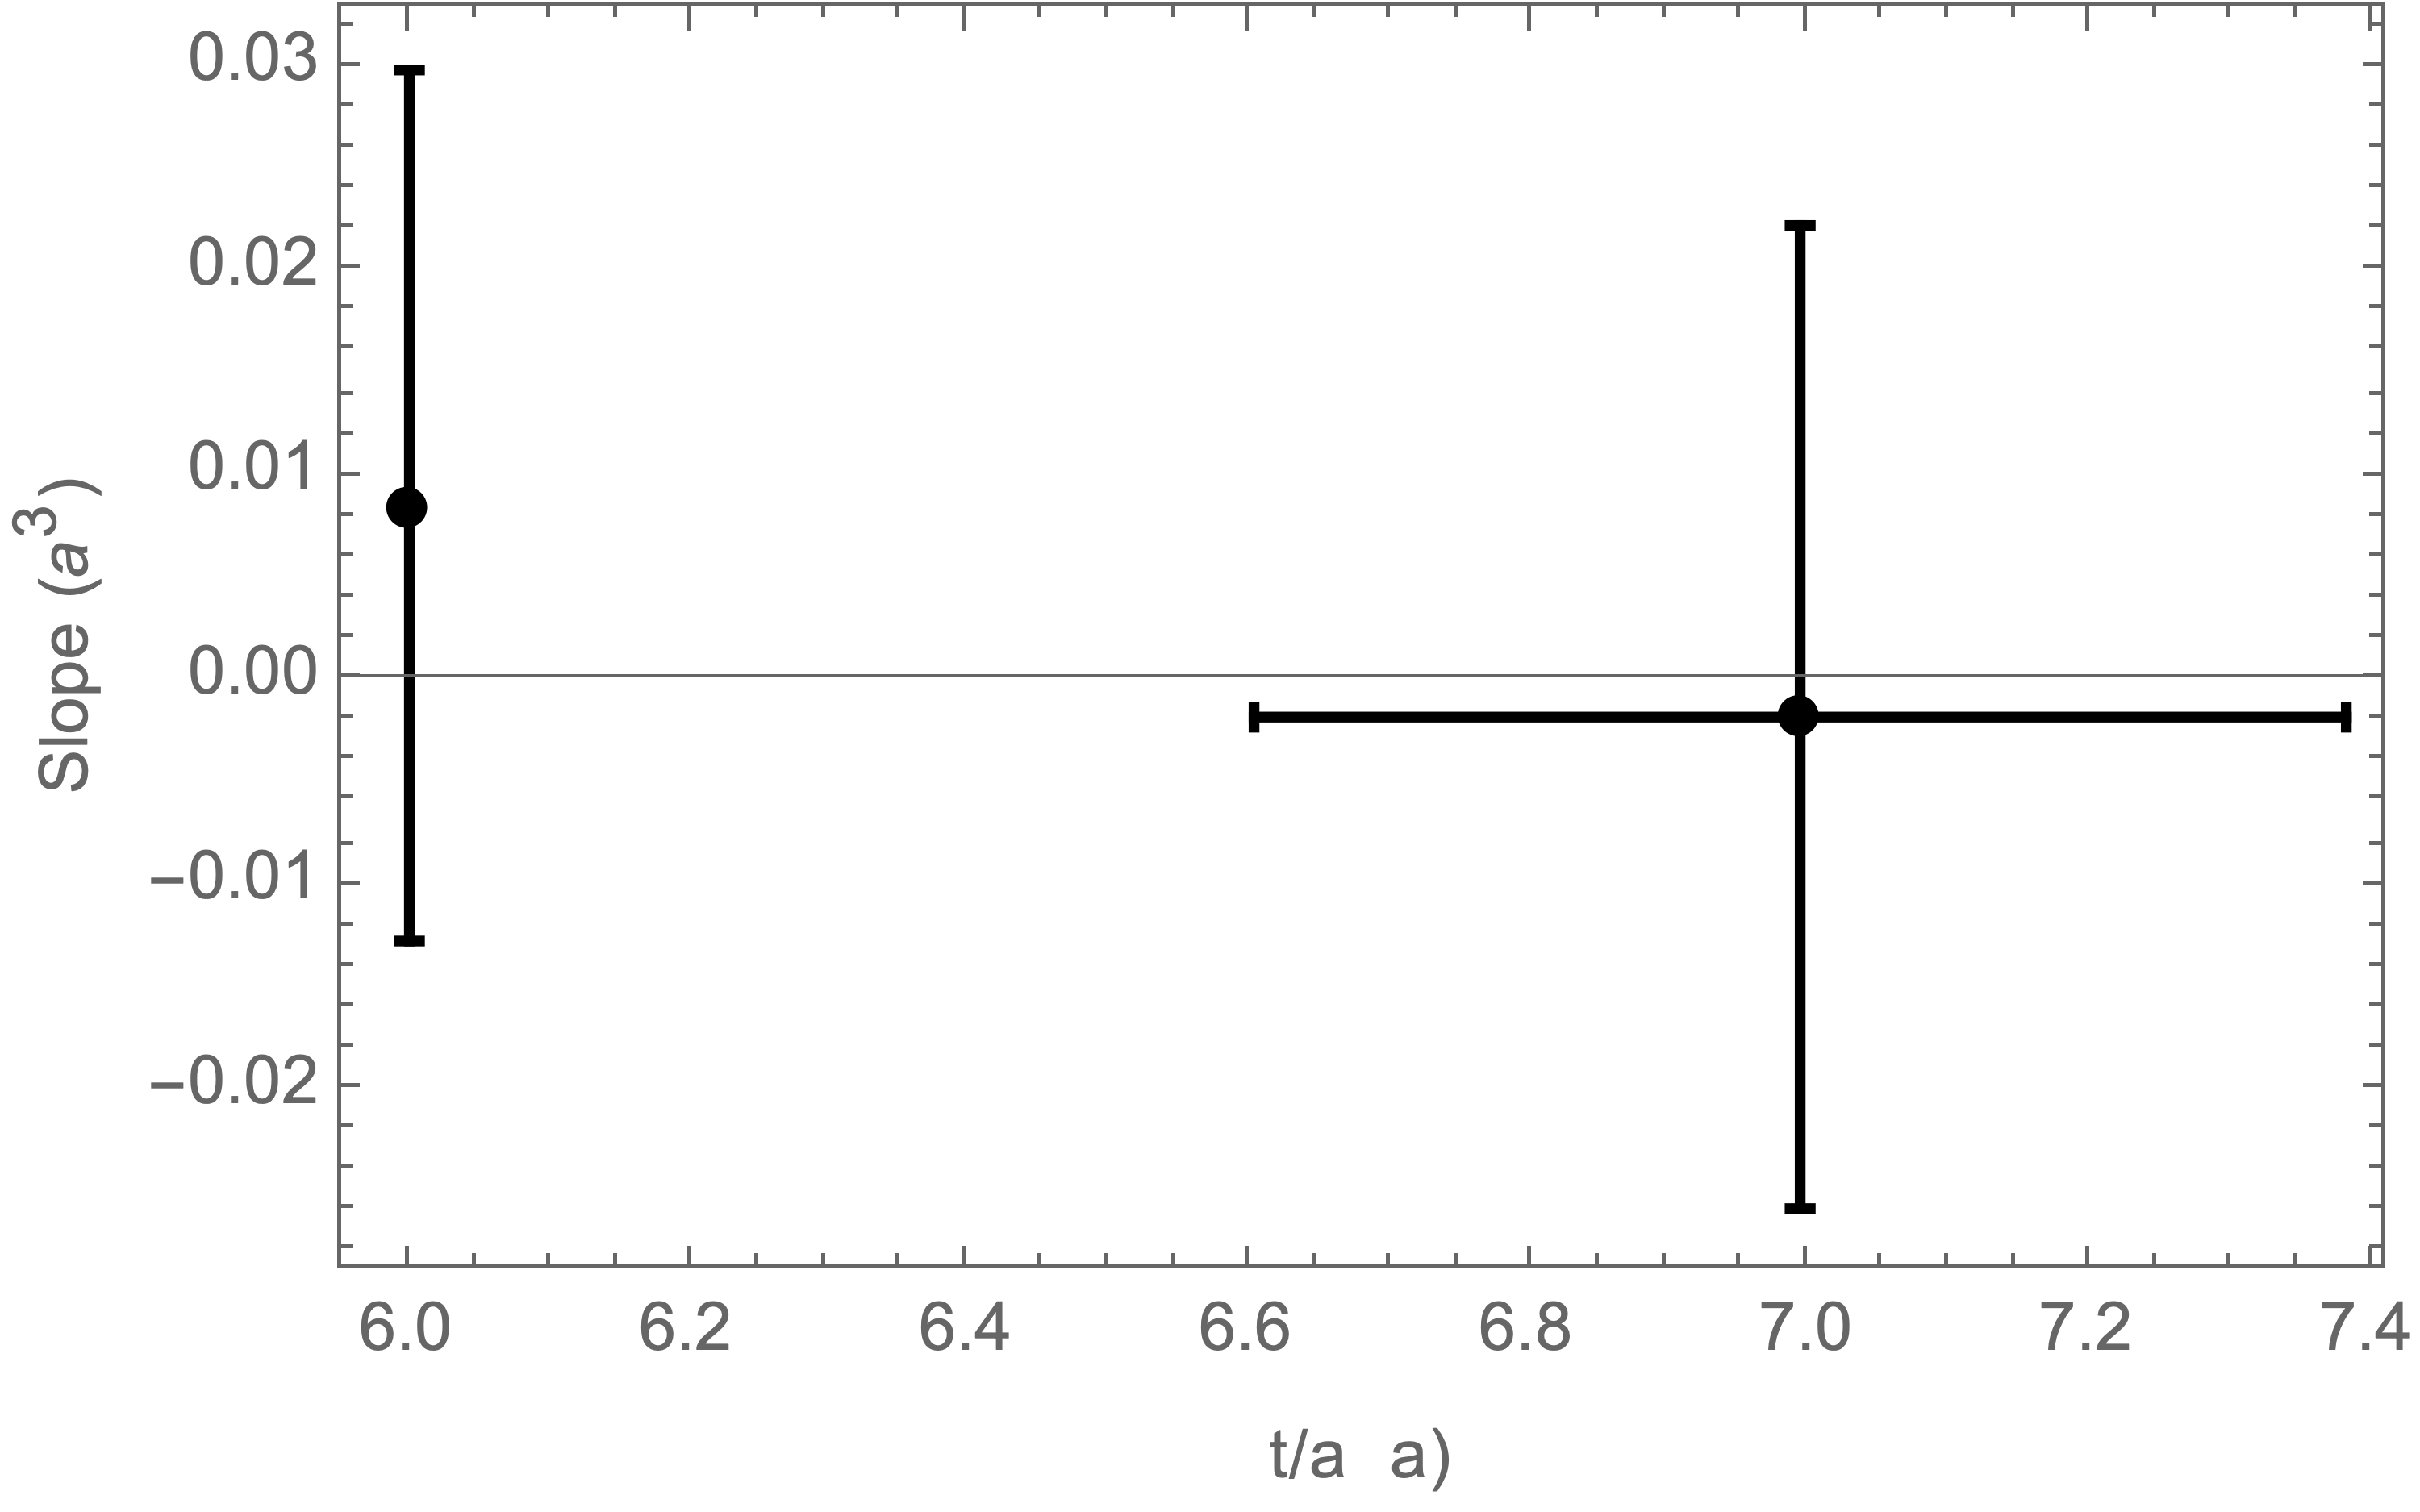
\includegraphics[width=.33\linewidth]{figures/3wF5-7Chi.png}
  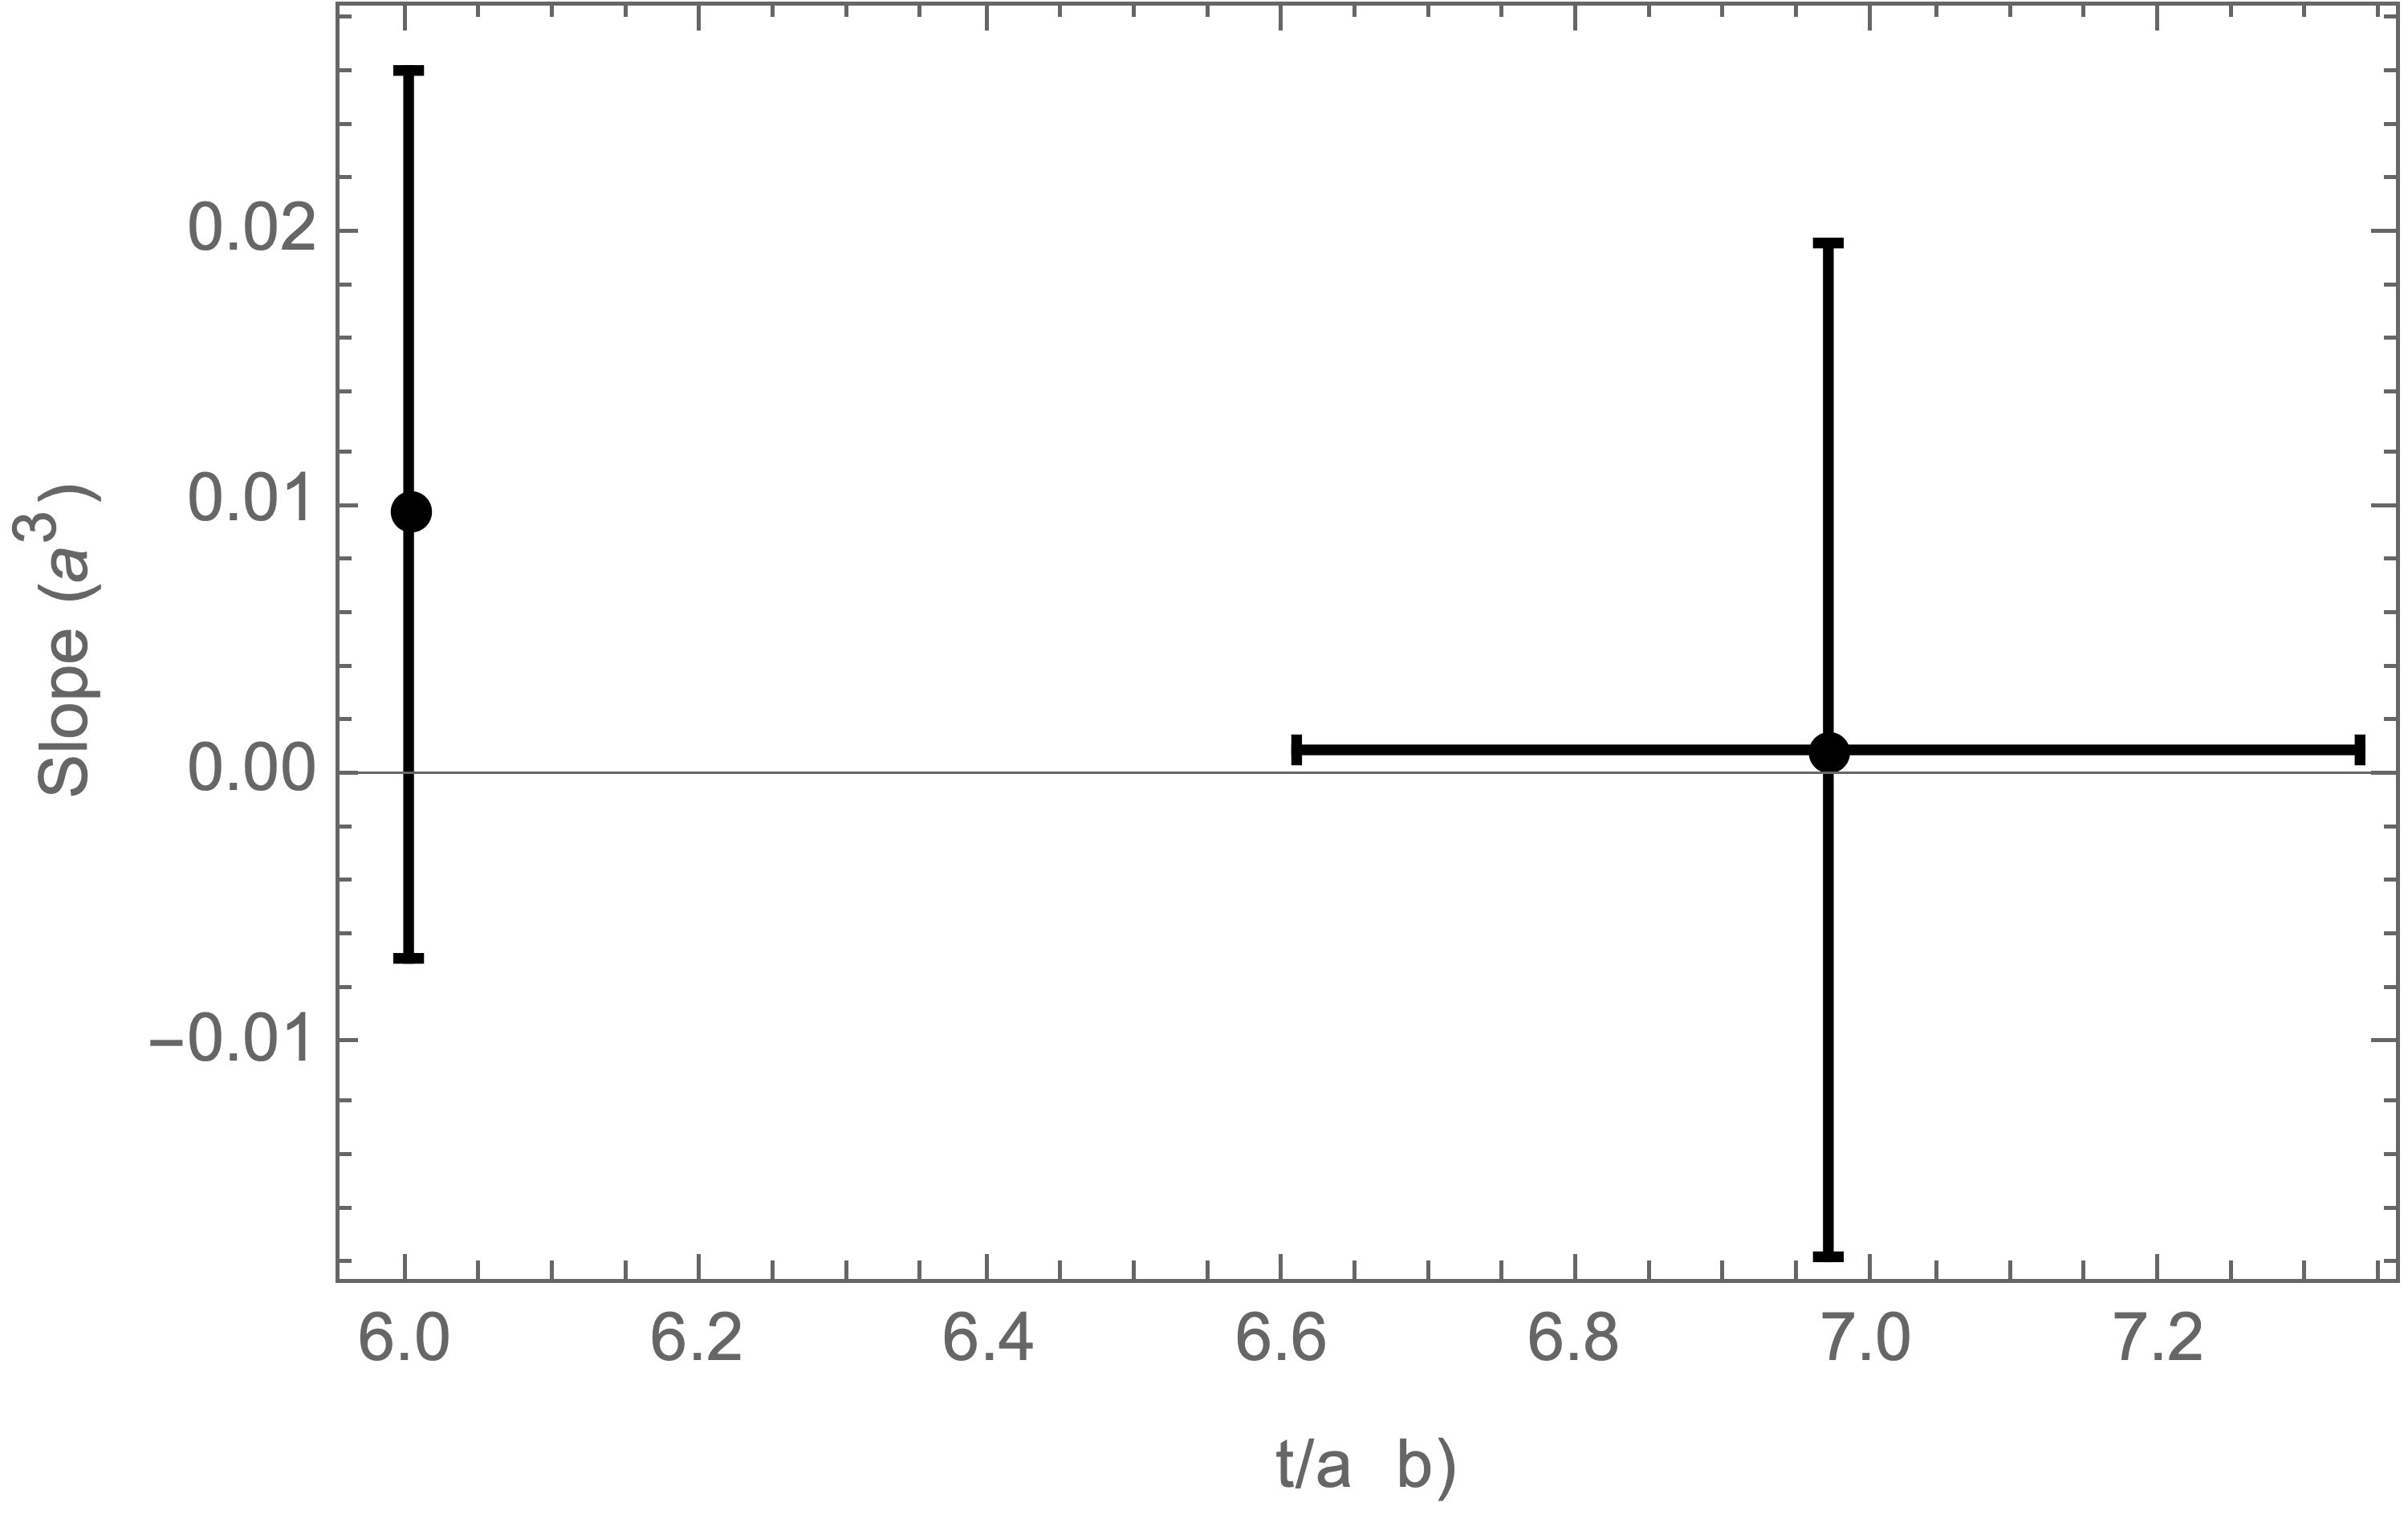
\includegraphics[width=.325\linewidth]{figures/3wF4-8Chi.png}
  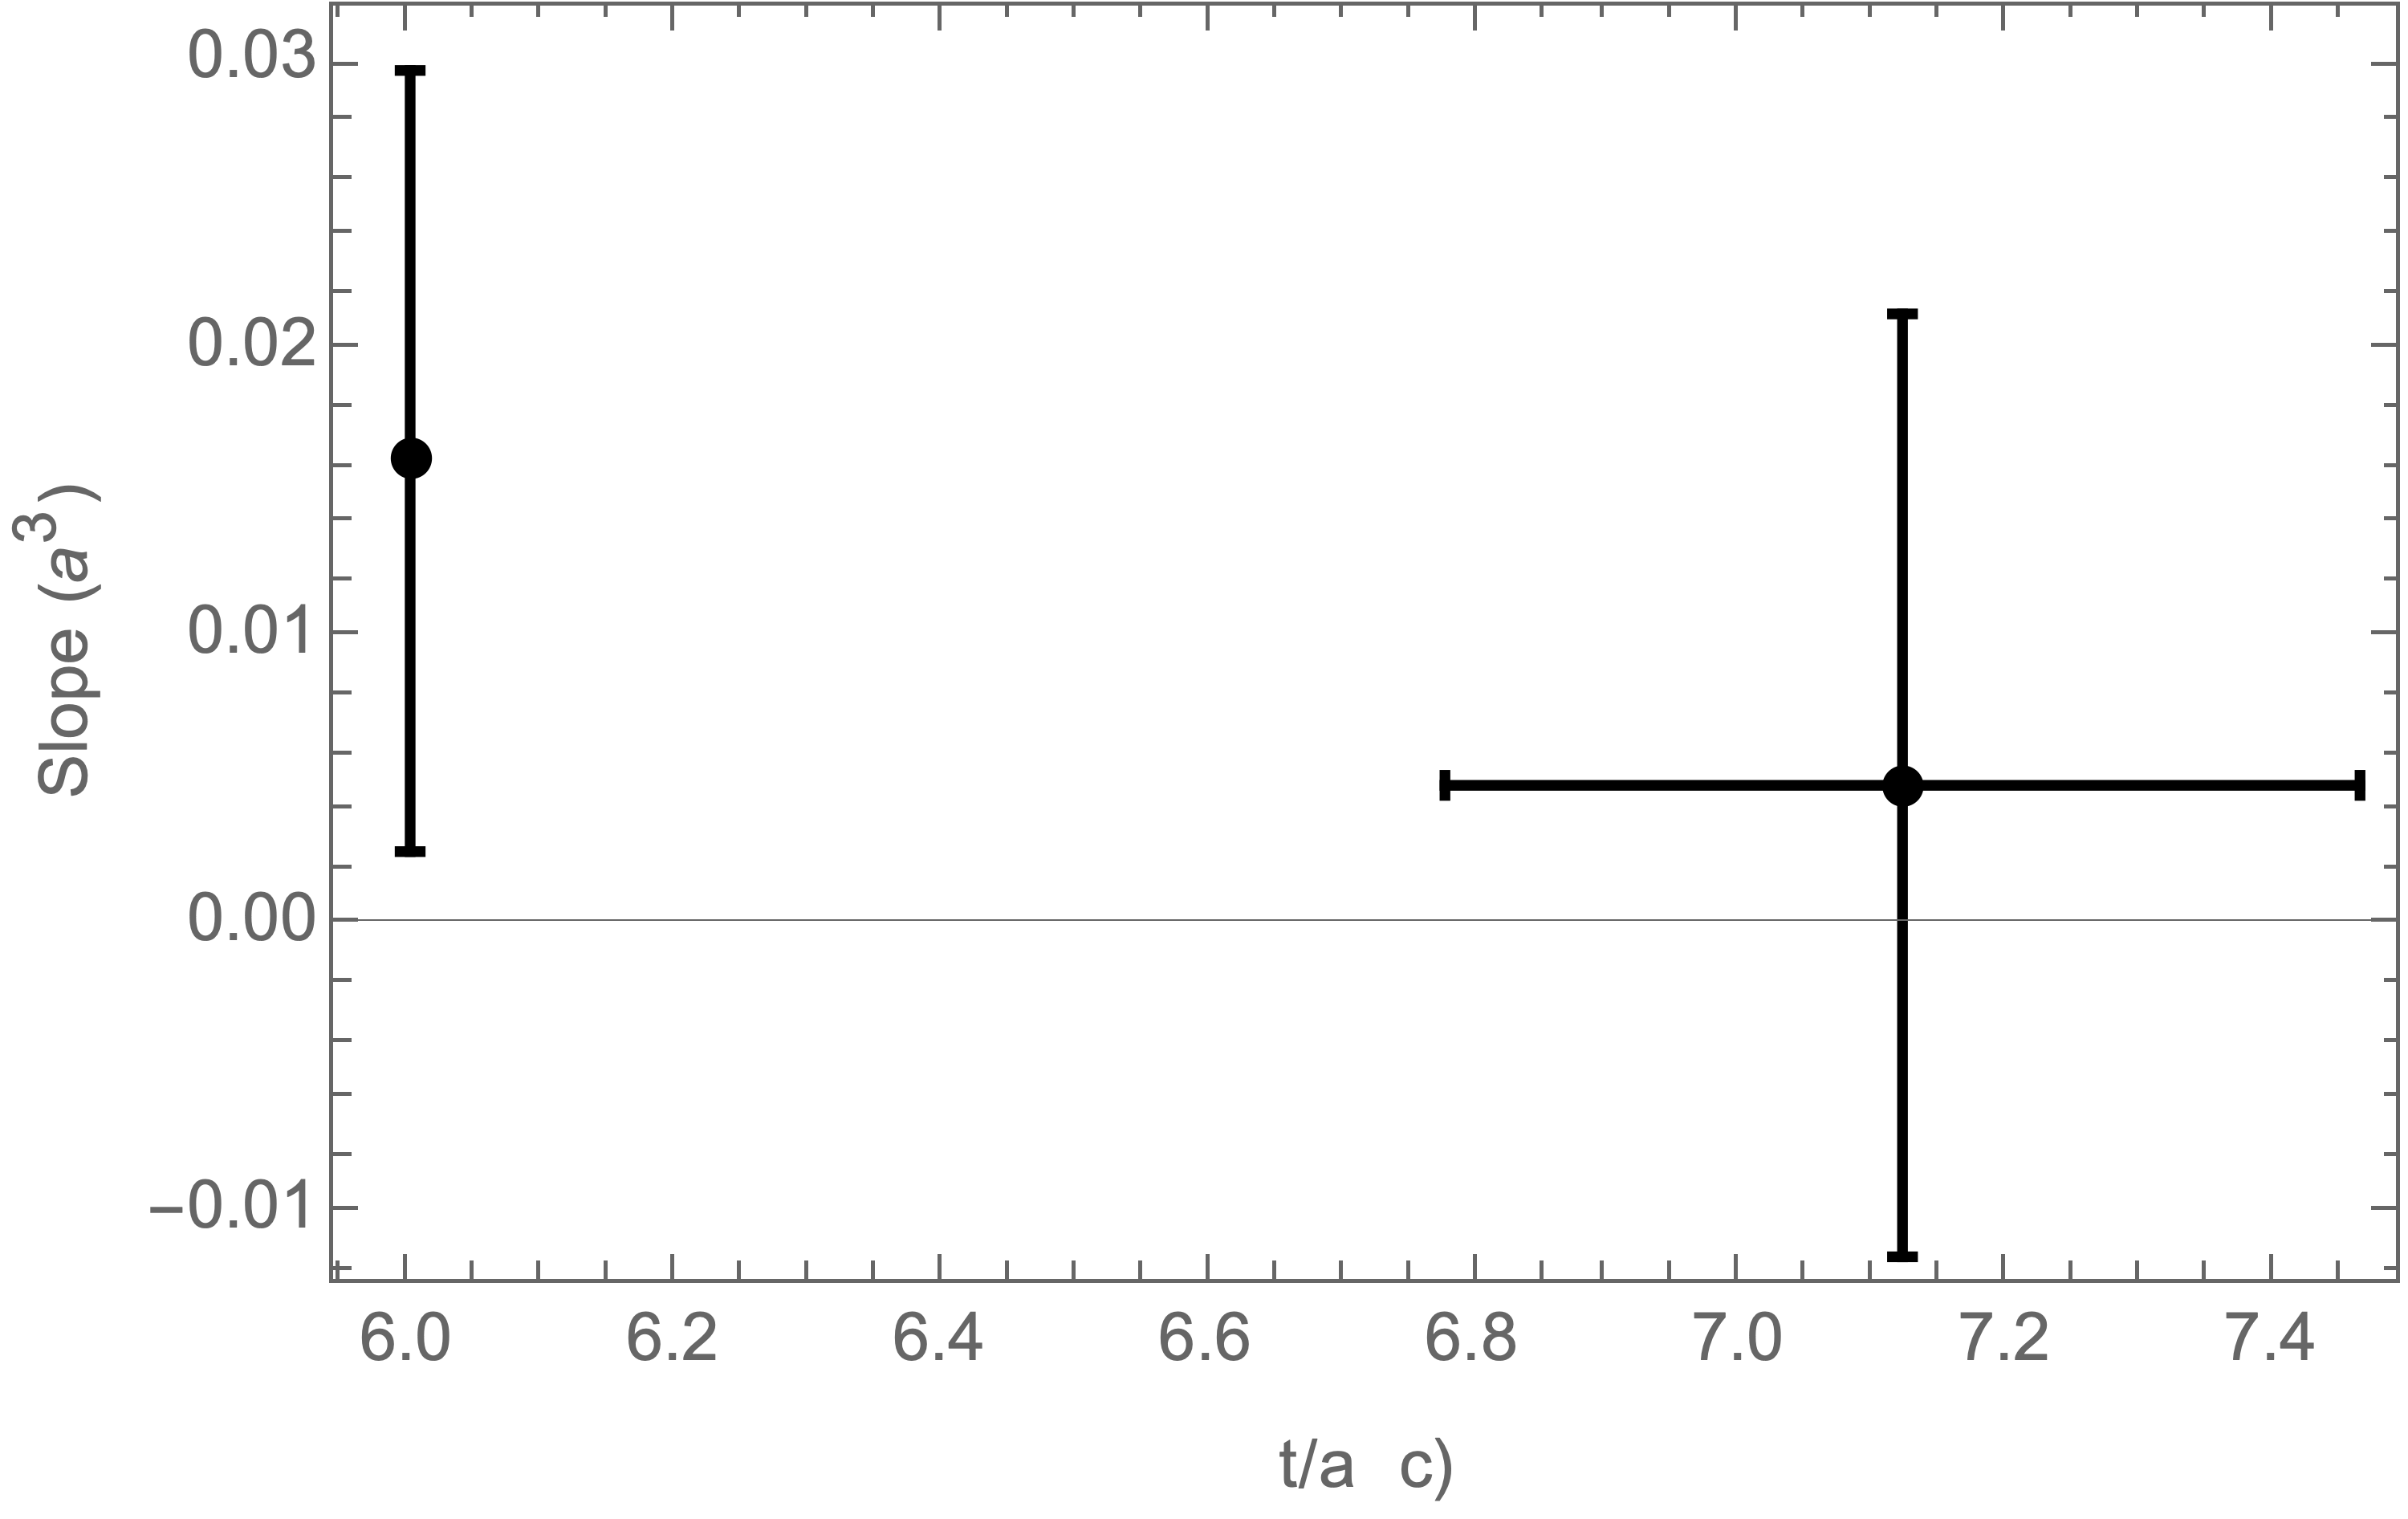
\includegraphics[width=.325\linewidth]{figures/3wF3-9Chi.png}
  \caption{Slope values at the shifted inflection points and at $t=6a$ for all diagrams. a) 5 to 7, 
  b) 4 to 8, c) 3 to 9 $\chi^2$ fitting ranges in the three-window analysis.}
  \label{fig:shiftinflec_all}
\end{figure}
In the $\chi^2$ quadratic fits, in the one-window analysis,  with and without a quadratic terms yield 
positions with a considerable uncertainty. However, the slopes at those points agree within uncertainties 
with those at the inflection point $t=6a$, c.f. table~\ref{tab:1walphaconnected} 
and figure~\ref{fig:1wshifinflec_all}.
\begin{figure}[H]
  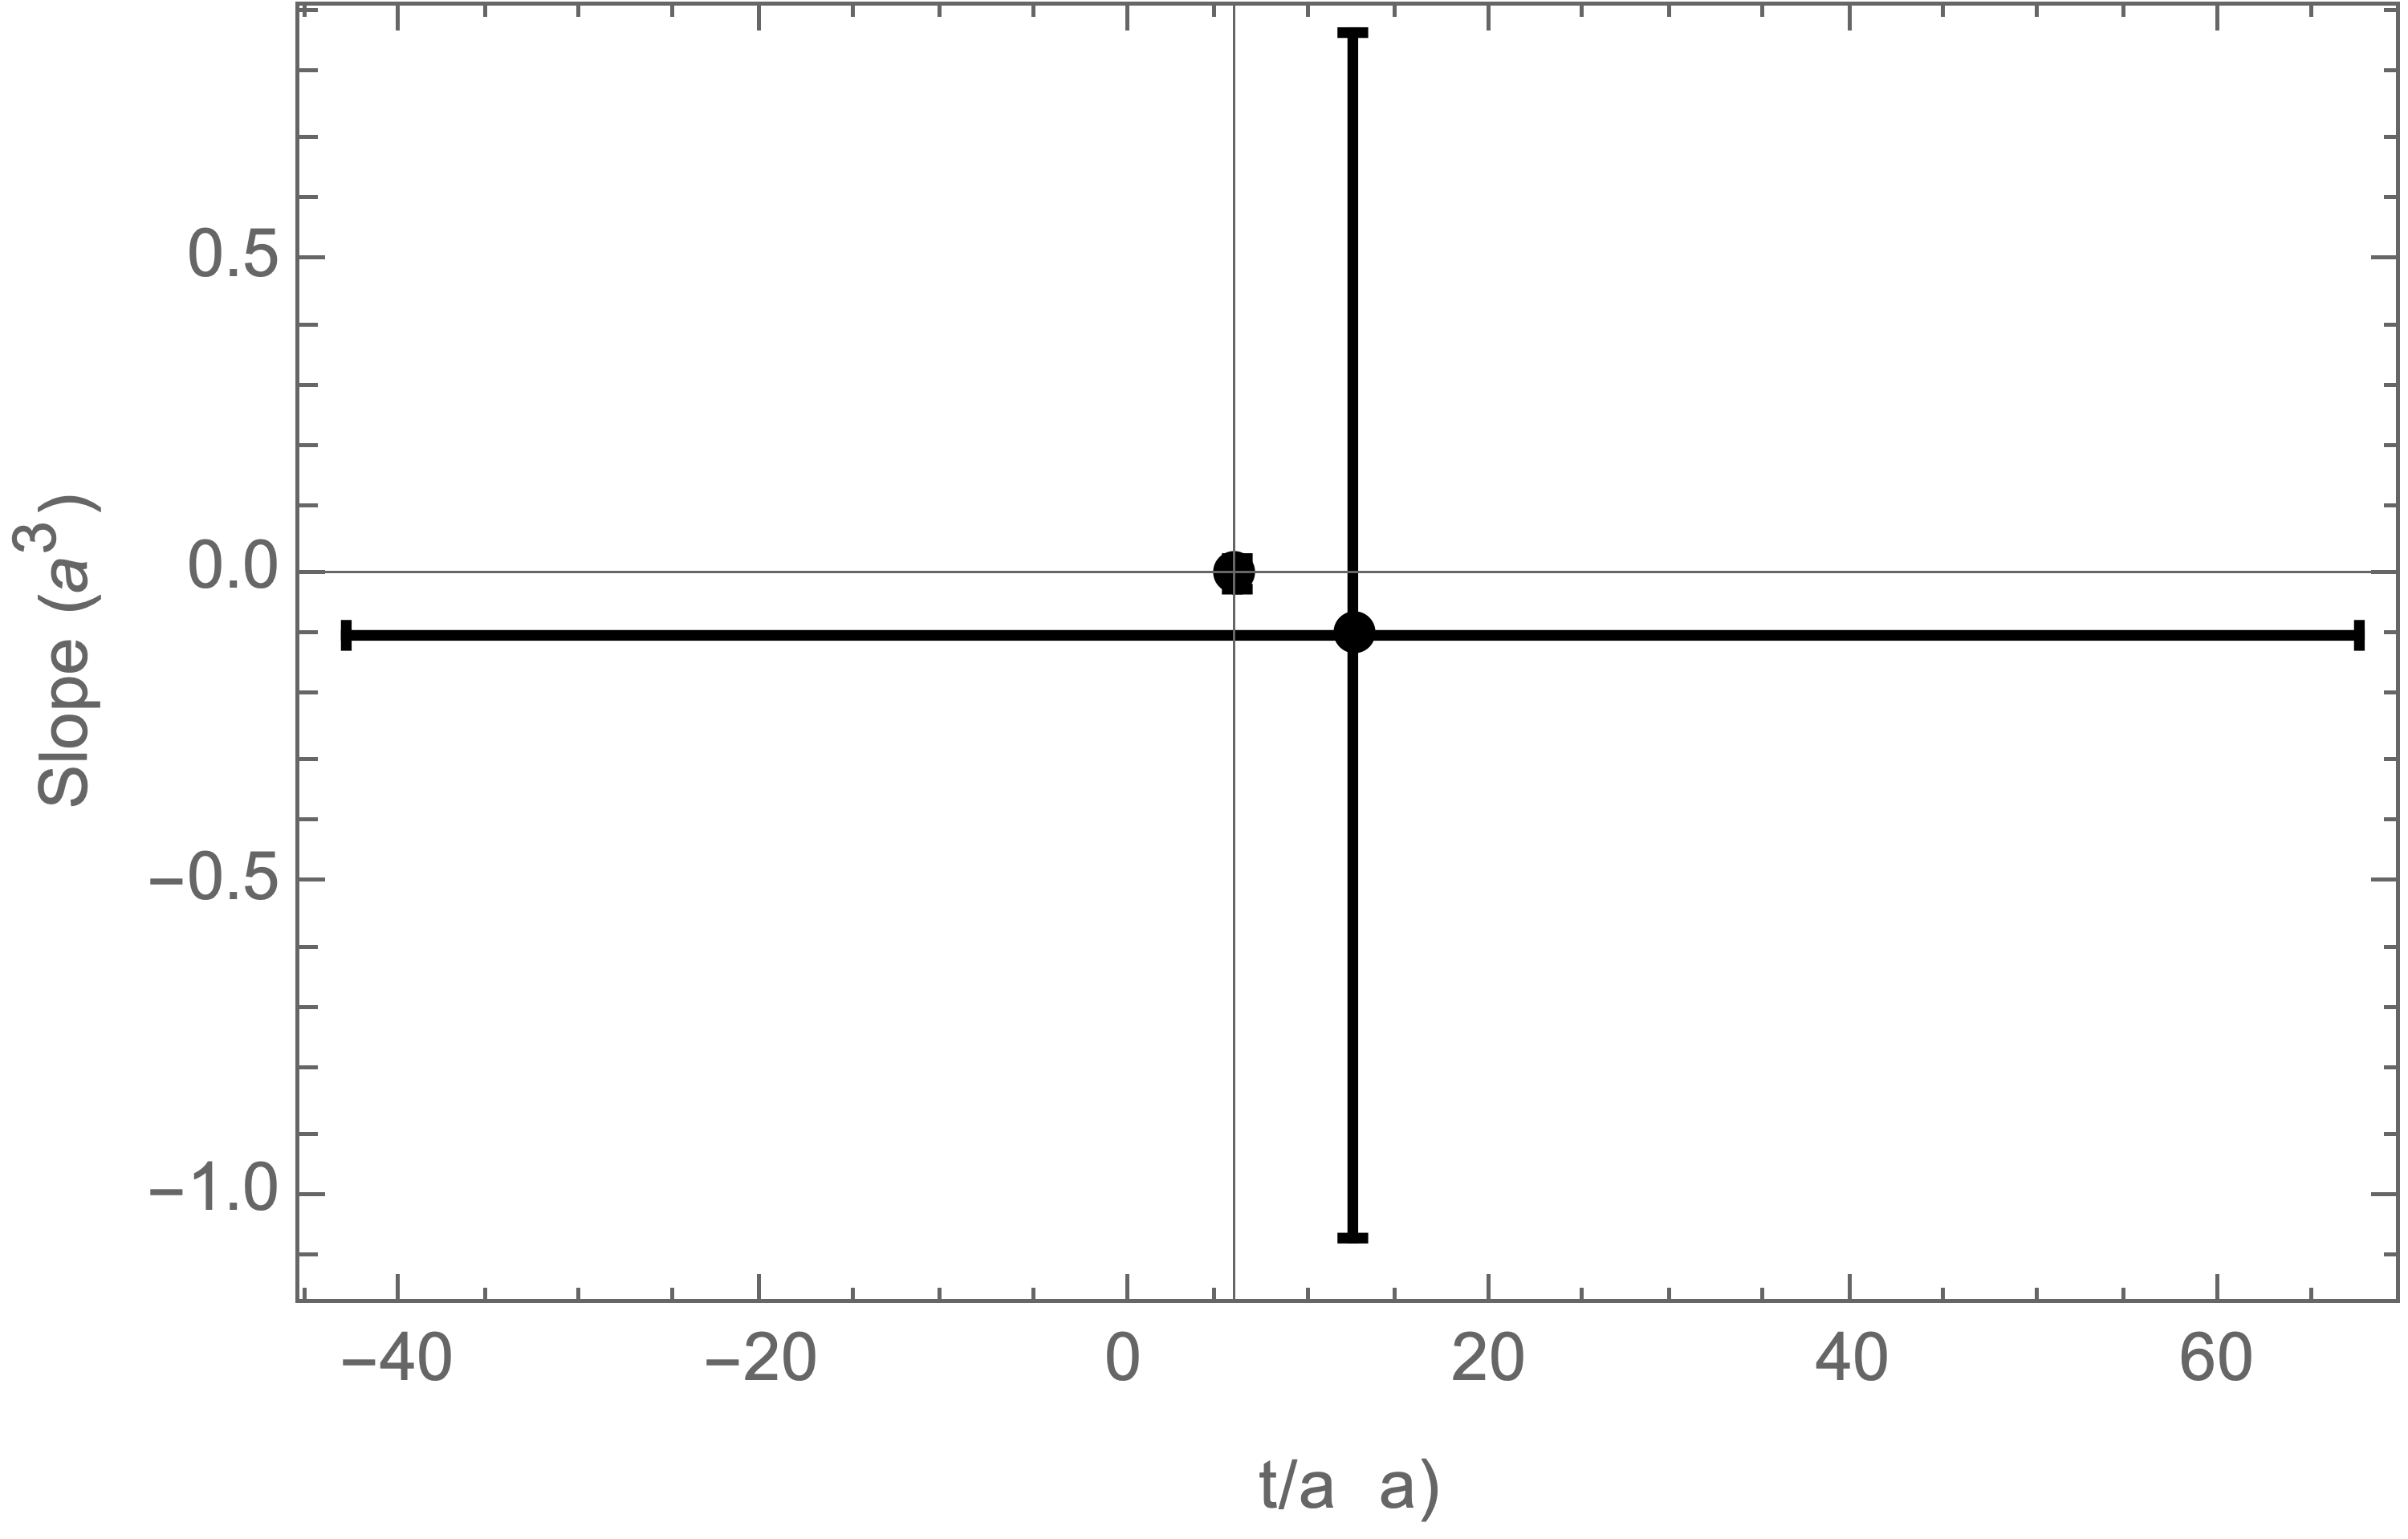
\includegraphics[width=.49\linewidth]{figures/1wF4-8Chi.png}
  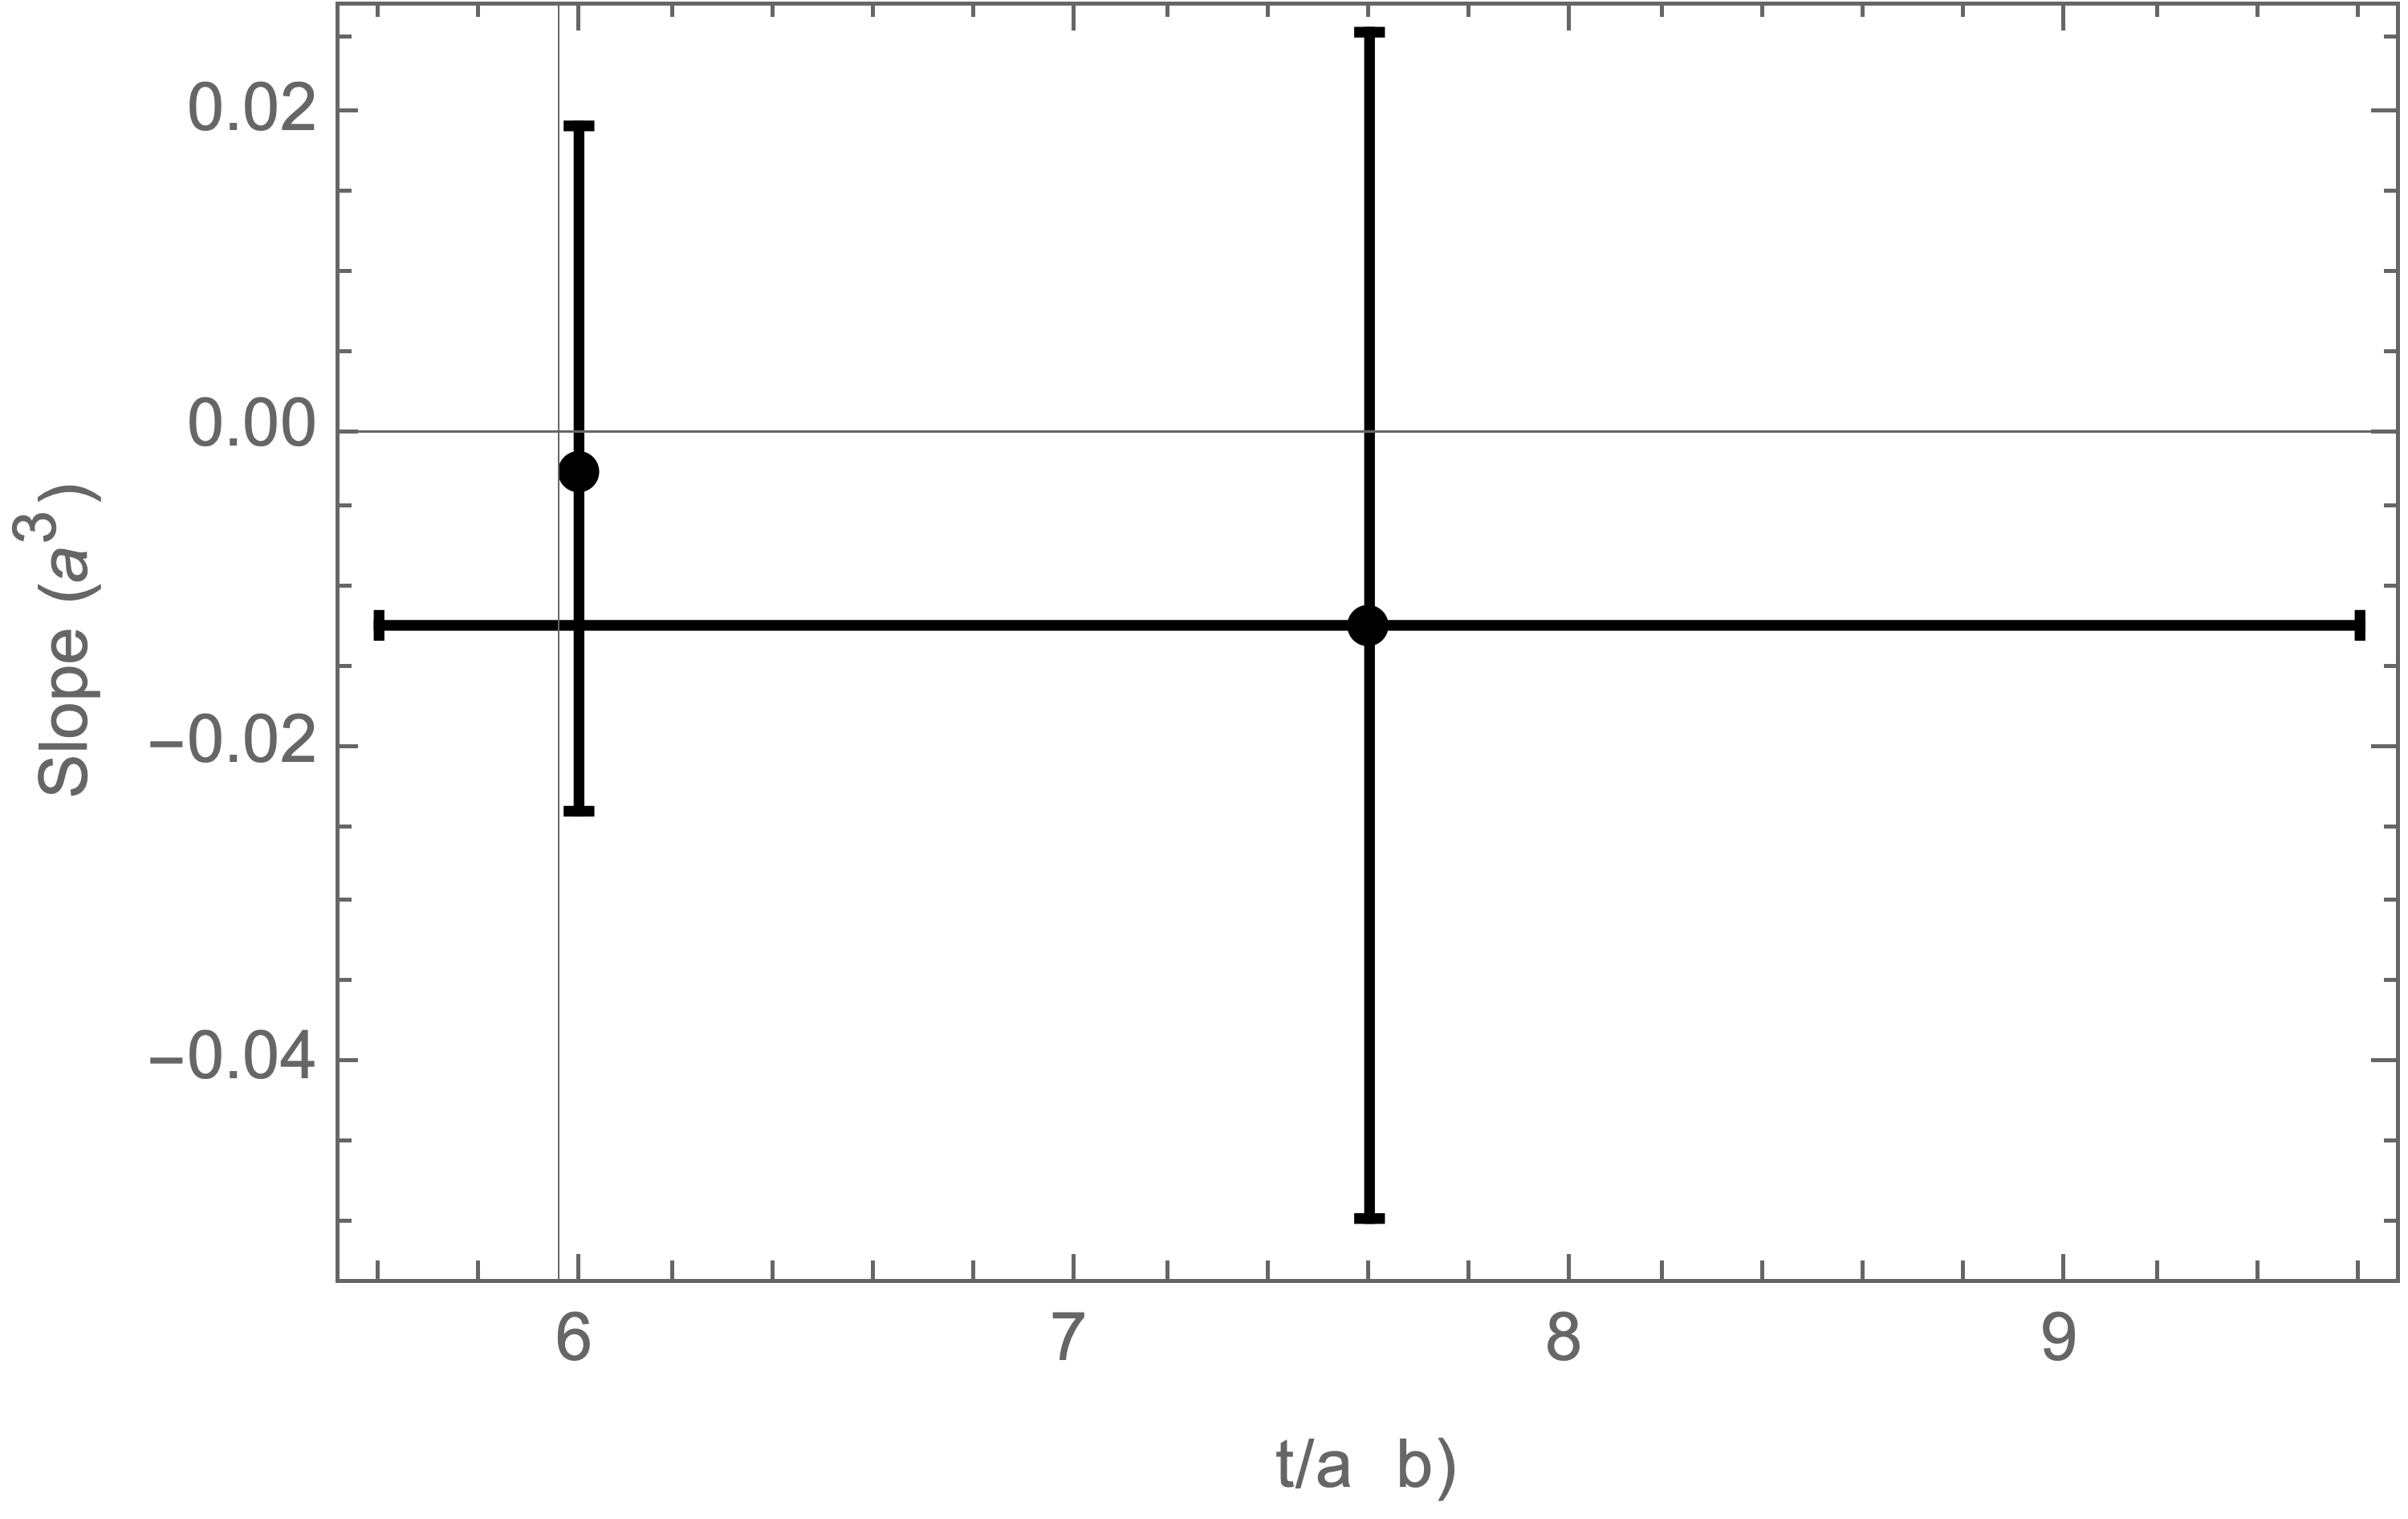
\includegraphics[width=.495\linewidth]{figures/1wF3-9Chi.png}
  \caption{Slope values extracted form the $\chi^2$ fitting ranges a) 4 to 8 and b) 3 to 9 for all diagrams
  in the one-window analysis.}
  \label{fig:1wshifinflec_all}
\end{figure}
The previous connected and all diagrams results show slopes at the inflection point consistent
with the slopes at $t=6a$. Although the 3-window analysis shows that the inflection 
points shift, the one-window analyses yield large uncertainties in their positions. The slopes at 
theses points are also consistent with the ones at the inflection points of construction $t=6a$. 
Consequently, we conclude that our results strongly suggest no excited-state analysis.